\chapter{Our method}

A synthetic 3D model has a canonical, continuous, and dense 2D parameterization which is not dependent the 3D model pose or deformation. Pose means the translation and rotation of the model, and deformation means the independent movement of the model vertices. We used the 3D model to render large quantities of randomized, deformed, and non-realistic training data. The training data consisted of randomized facial images and corresponding 2D parameterization images. Using this data, we trained a neural network to detect faces from images and to identify the pixels inside the faces with the 2D parameterization. This gave a 2D correspondence between the face pixels and the 3D model.

This chapter goes into the details of our method, and the chapter is divided into sections as follows:

\begin{itemize}
    \item Section \ref{sec:general_workflow}, general workflow, describes the repeated high-level work that was needed to iteratively improve the results.
    \item Section \ref{sec:uv_color_mapping}, UV color mapping, explains how we used the 2D parameterization of the head model for the geometry mapping.
    \item Section \ref{sec:syn_data_gen}, synthetic data generation, explains the details necessary to create a diverse enough training dataset.
    \item Section \ref{sec:net_design}, neural network design, shows the final topology of the network and the particular features of its layers.
    \item Section \ref{sec:loss_func}, loss function design, illustrates how the training sample flowed through the network and how the final loss value was calculated from the resulting images.
    \item Section \ref{sec:data_aug}, data augmentation process, details every augmentation method we used to increase the effective size of the training dataset, and especially how the occlusion augmentations were created.
    \item Section \ref{sec:training_process}, training process, presents the software architecture used for the training.
    \item Section \ref{sec:viz_methods}, visualization methods, details all the techniques we used to generate evaluation images from the network outputs.
    \item Section \ref{sec:results_eval}, results evaluation, explains the technical details behind managing the evaluation and inspection of a large number of training runs and result images.
\end{itemize}

\section{General workflow}
\label{sec:general_workflow}

Figure \ref{fig:workflow_1} depicts the general workflow of our method from a higher level. We started by editing the head model and associated materials in the \textcite{blender} 3D computer graphics toolset. After having adjusted rendering parameters, a test rendering was executed on the local computer. This usually took about one hour and in the end generated a large collage with hundreds of renderings combined. Using this collage, we then determined if further rendering adjustments were necessary. If they were, this adjust-render-evaluate method was repeated until the renderings looked satisfactory.

\begin{figure}
    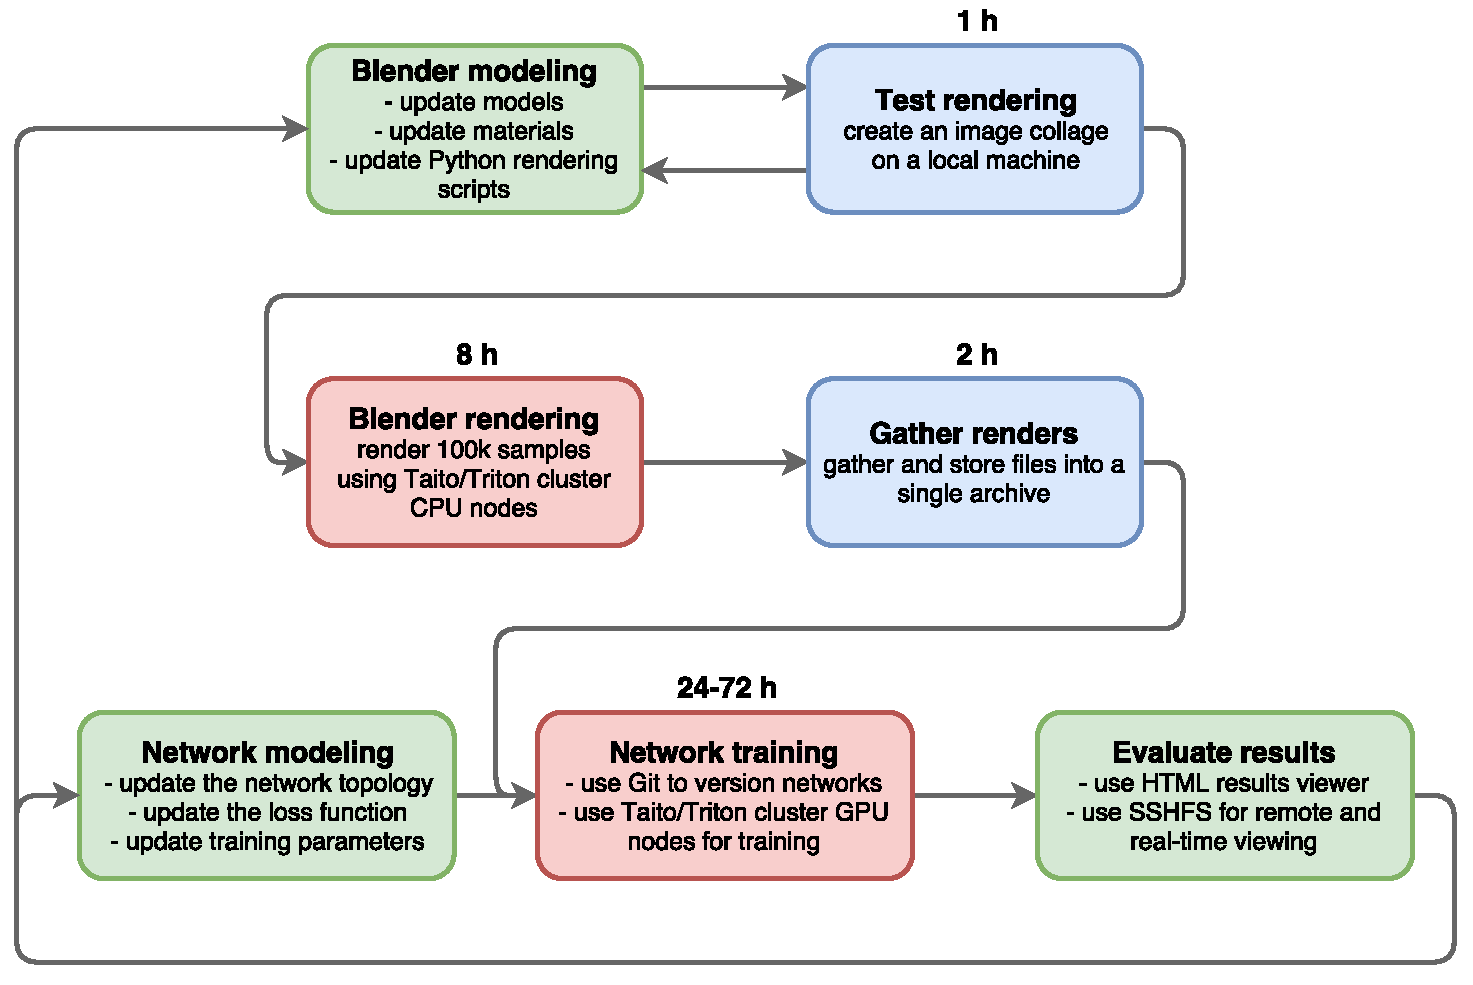
\includegraphics[width=\textwidth]{workflow}
    \caption[Research workflow]{Overview of our research workflow. Green boxes mean manual work that did not have an exact duration. Blue boxes mean small-scale non-parallel jobs. Red boxes mean massively parallel and long-running jobs on either the \ac{CPU} or \ac{GPU} nodes in the Aalto Triton or \ac{CSC} Taito computing clusters.}
    \label{fig:workflow_1}
\end{figure}

Updated rendering related files and scripts were then uploaded to the Aalto Triton or \ac{CSC} Taito computing clusters. There, a massively parallel rendering job was launched that generated 300 000 individual rendered images. The job took on average eight hours to finish. This big set of files was then gathered together and compressed into a single archive, taking over 10 gigabytes of storage space.

While the rendering was underway, we manually tuned the neural network parameters. The validity of the changes was tested on a local computer using quick test runs. We created up to 20 different training configurations where usually a single change was made to either network, loss, or augmentation parameters. After the training dataset generation had finished, we sent it together with 20 different training jobs to the \ac{GPU} nodes in the computing cluster.

After the models had been under training for a maximum of three days, we started to evaluate the results. The evaluation was done by mounting the result directory to a local computer using \ac{SSHFS} and then looking at the generated evaluation images using the custom-made browser-based viewer. We compared the results from all the 20 different jobs visually and by using some simple evaluation metrics. After we had come to conclusions with the current results, we started the process from the beginning by going back to updating the network and rendering models. In the end, this process was repeated about 15 times which means that around 300 24--72 hour training runs were performed.

\section{UV color mapping}
\label{sec:uv_color_mapping}

\begin{figure}[h]
    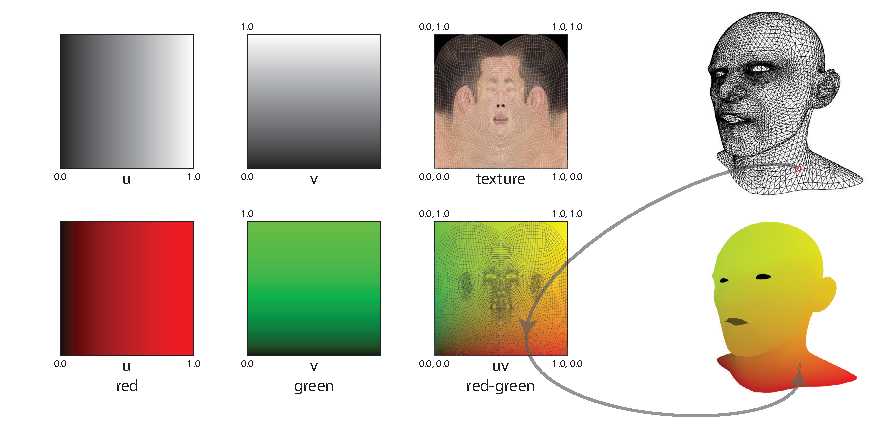
\includegraphics[width=\textwidth]{uv-color-mapping}
    \caption[UV color mapping]{UV color mapping. Same idea as in texture mapping but the texture is replaced by the procedural color representation of the UV coordinates. The 3D triangle mesh is ''opened up`` and flattened to the 2D UV space so that the triangles do not overlap.}
    \label{fig:uv_color_mapping_1}
\end{figure}

The key insight to our method is understanding the UV color mapping we used. Figure \ref{fig:uv_color_mapping_1} illustrates this idea. A 3D model consists of triangles, and each triangle has three vertices. These vertices each have at least two attributes: a 3D world position and a 2D UV coordinate. The position can have any arbitrary values, but the UV coordinate is constrained to values between 0.0 and 1.0. It could be thought that the 2D UV values are real-valued positions on a square whose side length is 1.0. When a 3D model is created, its UV mapping is generated at the same time automatically with some manual tuning afterward. The UV map generation can be visualized as opening the 3D model up and then warping and flattening the triangles onto the 2D UV square. The flattening is done so that the triangles do not overlap in the UV space, that is, each triangle is mapped to a unique area. After the UV mapping has been done, it does not change even if the 3D world positions of the model vertices are changed. The change could be caused by, for example, expression animation or by applying scaling or deformation operations to the 3D model. Figure \ref{fig:uv_color_mapping_1} illustrates the UV dimensions both in grayscale and with color; red for the U dimension and green for the V dimension. If these separate color channels were combined, it would result in a color gradient shown in the red-green square. The color choice has been arbitrary; it affects only on the visualizations of the results.

Usually, the UV mapping is used to texture the 3D model using textures like one in the texture square of figure \ref{fig:uv_color_mapping_1}. We replaced this normal texture with the red-green-yellow gradient texture generated procedurally straight from the UV coordinates. This resulted in the red-green-yellow renders of heads as seen in, for example, figure \ref{fig:head_final_triplet_collage_1}. Looking at a render like that, each pixel of the head tells precisely where that pixel belongs to in the UV space. Now, if we can generate this same UV color mapping from an arbitrary face image, we can then use the mapping to sample textures, create own visualizations using static or procedural textures, swap faces between two people, or recreate the 3D mesh of the face.

Many corresponding input and UV images can be rendered using just one head model while deforming it in many ways. Even if the appearance the model changed, the UV mapping would stay the same. These input and UV image pairs can then be used to train a neural network to do the mapping. The network can become invariant to facial geometry changes and would be able to map very different facial geometries to the same underlying UV mapping.

\section{Synthetic data generation}
\label{sec:syn_data_gen}

For generating the images in the training dataset, we decided to use \textcite{blender}. The choice was quite easy, as Blender is free and open source, and it has comparable features to commercial 3D modeling software. In addition, Blender comes with the Cycles rendering engine which has all the features we needed. We could use the nodes material system to design arbitrary materials and output resulting renders in multiple file formats. Blender is heavily based on the Python scripting language, and that allowed broad access to the internals of the program with the use of external scripts. This meant that we could completely automate and randomize the rendering process from start to finish. Finally, blender supports Linux and running from the command line without opening a \ac{GUI}, which meant the rendering of a lot of images could be parallelized on a computing cluster.

\begin{figure}
    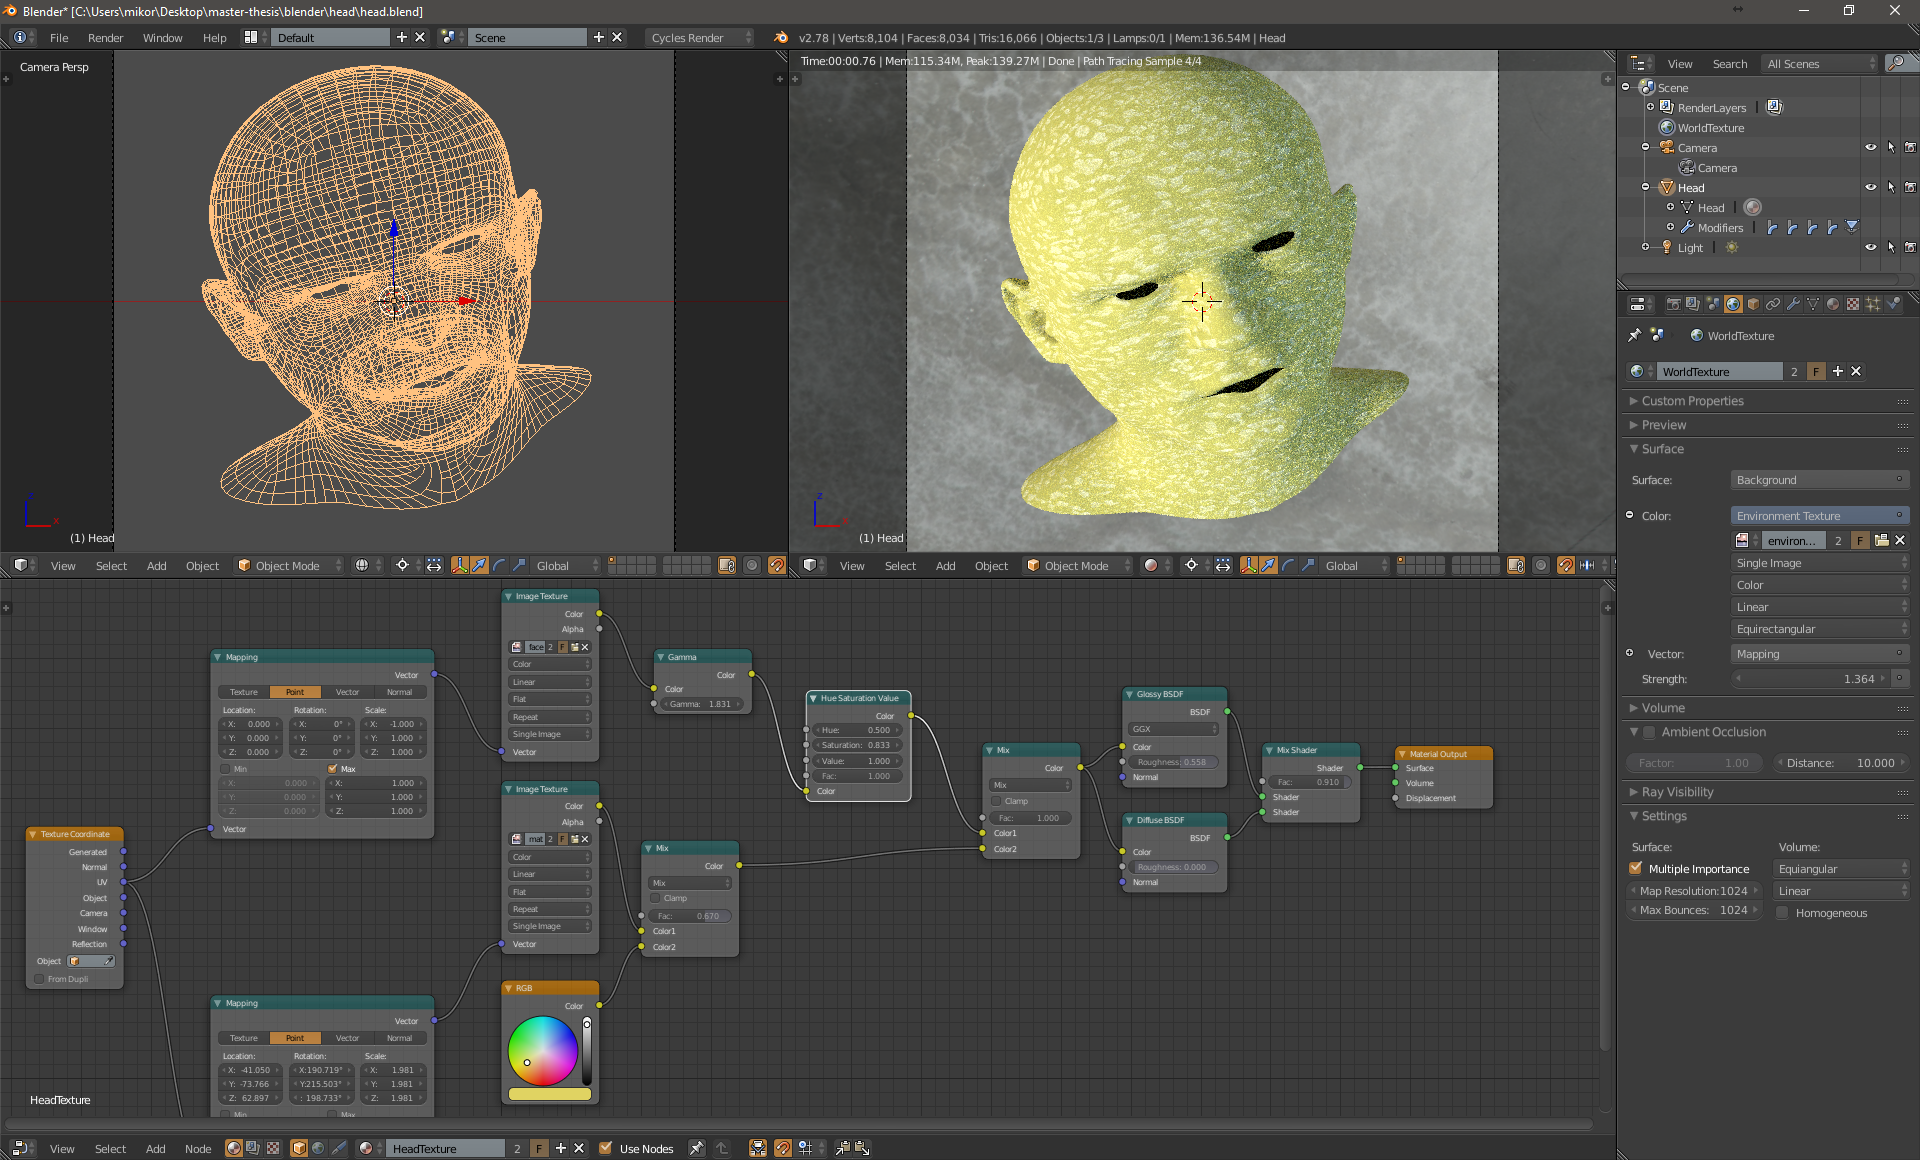
\includegraphics[width=\textwidth]{blender_edit_view}
    \caption[Blender modeling session]{A Blender modeling session. On the top left is the wireframe of the model, on the top right is the rendering result, and on the bottom is the current material modeled with the nodes system.}
    \label{fig:blender_edit_view_1}
\end{figure}

We received the head model and its textures from Remedy Entertainment. The dataset also contained 178 different expressions for the head model. A basic scene with the head, single directional light, and a background was set up. Materials for the head and background were designed using the Blender nodes system for materials. See figure \ref{fig:blender_edit_view_1} for an example of a typical editing session.

\begin{figure}
    \subfloat{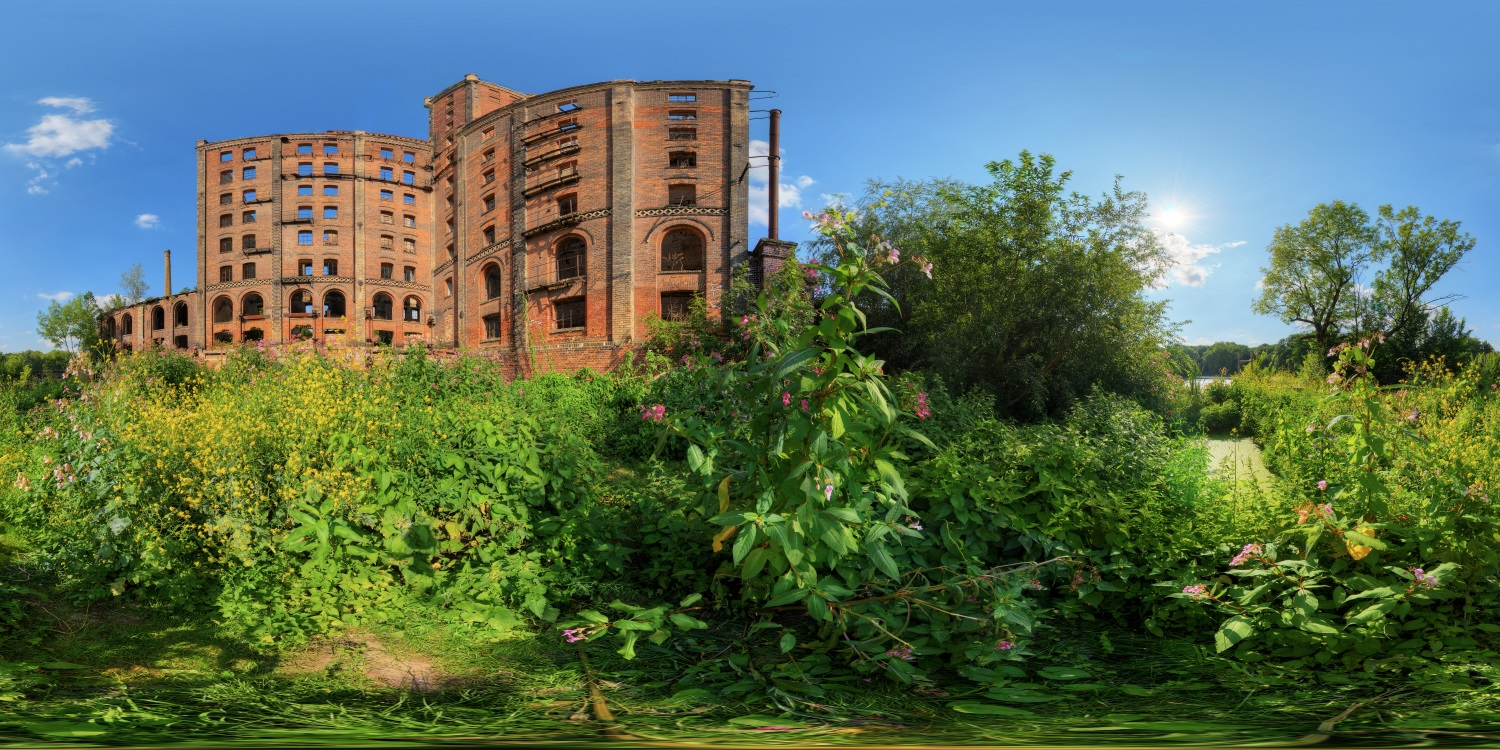
\includegraphics[width=\textwidth]{env_1}}\hfill
    \subfloat{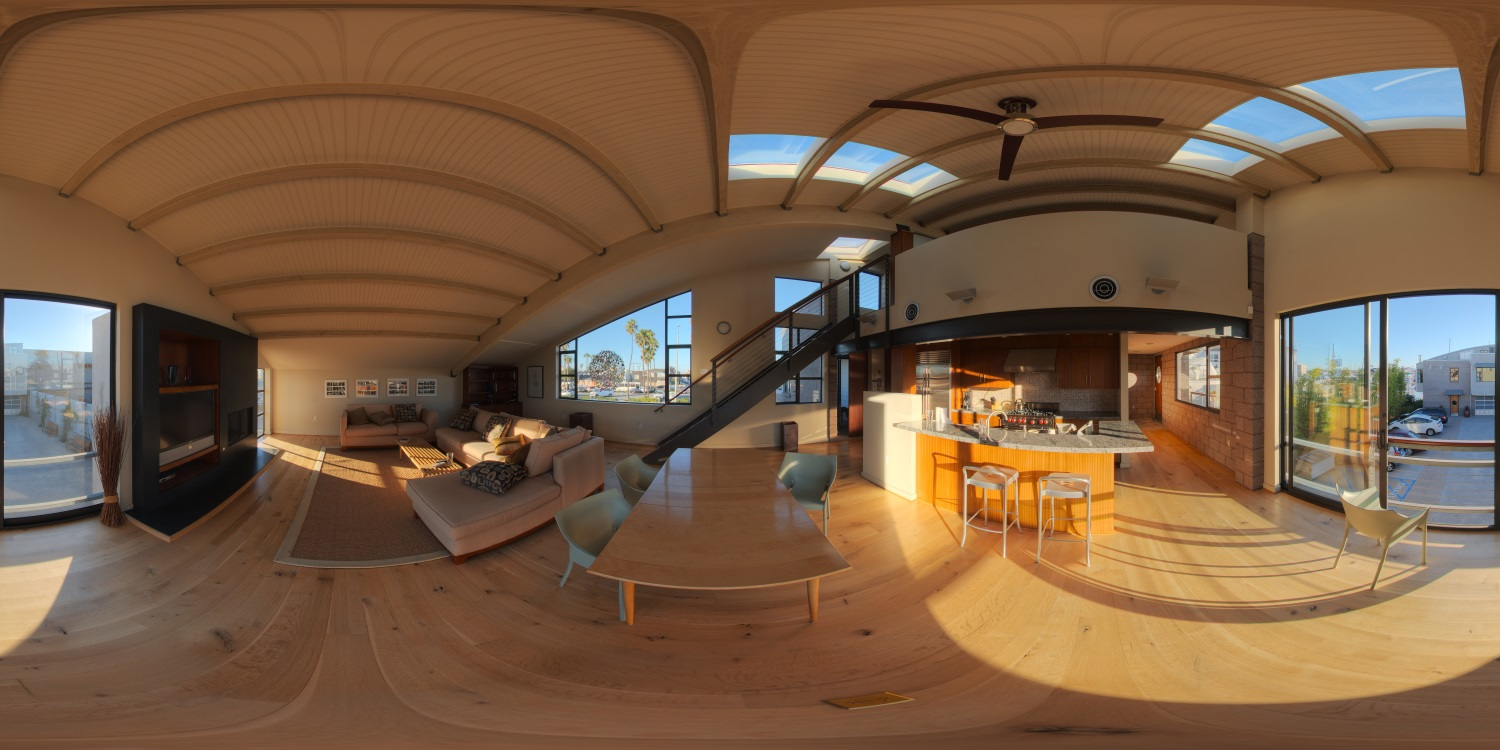
\includegraphics[width=\textwidth]{env_2}}\hfill
    \caption[Environmental textures]{Two examples of environmental textures with equirectangular projections. These were used for backgrounds when rendering and for generating occlusion masks when augmenting.}
    \label{fig:env_1}
\end{figure}

For the realistic backgrounds, we obtained 50 \ac{HDR} environment textures with a resolution of 8000x4000 from \textcite{sibl}. These textures had equirectangular projections, which meant that they could be projected 360 degrees around the head model without distortion. Two samples of environment textures can be seen in figure \ref{fig:env_1}. For non-realistic face textures, 70 different textures, with an average resolution of 1600x1600, were obtained from \textcite{textures}. Most of these textures were of natural materials and some were completely synthetic. Examples of these material textures can be seen in figure \ref{fig:face_textures_1}, along with the realistic face texture and the 1/f noise texture.

\begin{figure}
    \subfloat[Realistic texture]{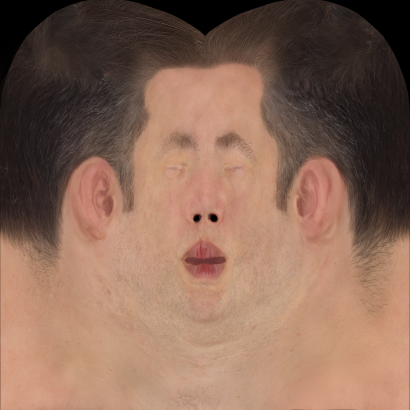
\includegraphics[width=.48\textwidth]{face_texture_1}}\hfill
    \subfloat[1/f noise texture]{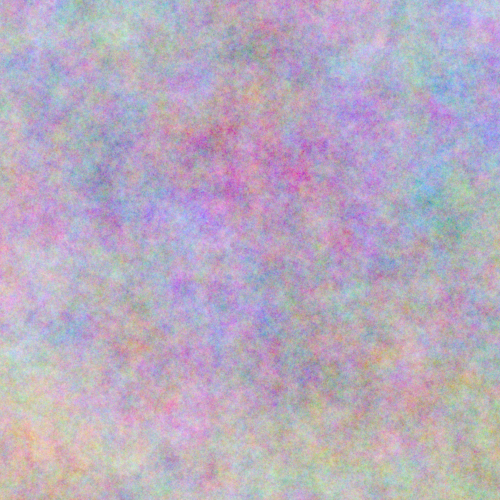
\includegraphics[width=.48\textwidth]{noise_1}}\hfill
    \subfloat[Material texture 1]{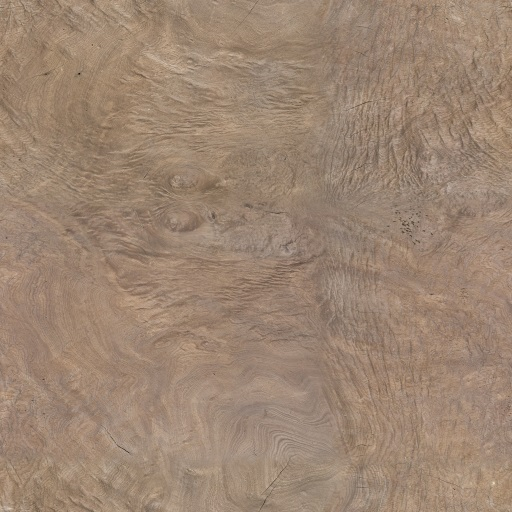
\includegraphics[width=.48\textwidth]{face_material_1}}\hfill
    \subfloat[Material texture 2]{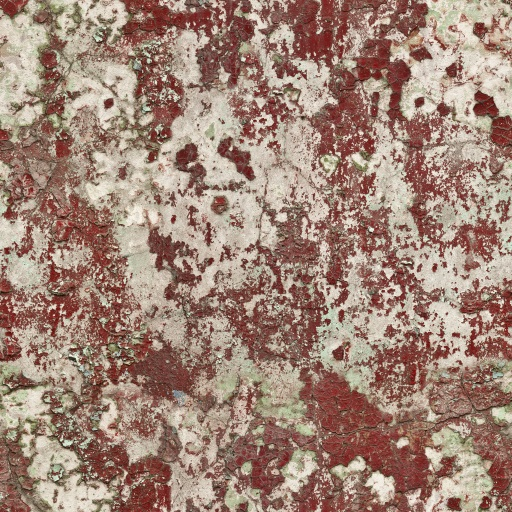
\includegraphics[width=.48\textwidth]{face_material_2}}\hfill
    \subfloat[Material texture 3]{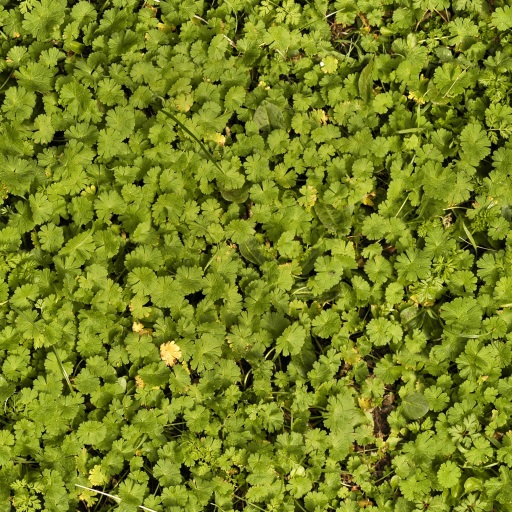
\includegraphics[width=.48\textwidth]{face_material_3}}\hfill
    \subfloat[Material texture 4]{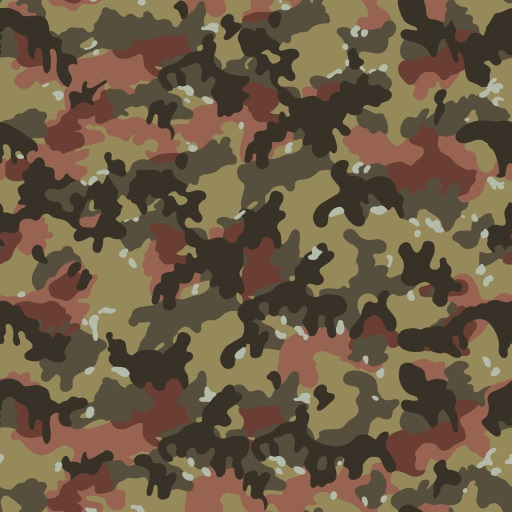
\includegraphics[width=.48\textwidth]{face_material_4}}\hfill
    \caption[Head model textures]{A sample of different textures used for rendering the head model.}
    \label{fig:face_textures_1}
\end{figure}

We started with very simple gray renderings (see figures \ref{fig:head_gray_1} and \ref{fig:head_gray_collage_1}) and then proceeded to more complex materials as it became evident that with the simpler materials it was not possible to successfully train the network. The idea behind using the 1/f noise textures (see figures \ref{fig:head_noise_1} and \ref{fig:head_noise_collage_1}) was that the 1/f noise follows the power spectra of natural images \cite{Schaaf1996}. The results were not that good, and we further experimented with different kinds of materials: completely realistic and completely non-realistic (see figures \ref{fig:head_material_texture_1} and \ref{fig:head_material_texture_collage_1}). In the end, we ended up with a head material that was a mixture of realistic face textures and non-realistic material textures. The material texture was first blended with a random solid color, and this blend was further blended with a realistic face texture. The blending amounts were also randomized. The actual \ac{BRDF} of the head material was a random blend between diffuse and glossy \acp{BRDF}. Samples of images with these blends can be seen in figure \ref{fig:head_final_texture_collage_1}. This figure also has the final amount of randomization in all the rendering parameters. Here is a detailed list of all the randomizations we did per each rendered training sample:

\begin{itemize}
    \item The head model scale was randomized in all three dimensions separately using a uniform random distribution.
    \item The head model rotation was randomized around all three axes separately using a Gaussian random distribution with zero mean. The standard deviations were set so that the 99.9th percentiles of the angles were as follows: pitch angle $\pm\ang{40}$, roll angle $\pm\ang{45}$, and yaw angle $\pm\ang{90}$.
    \item The head model was randomly deformed with Blender's simple deform modifiers of twist, bend, taper, and stretch.
    \item The head model was randomly deformed with Perlin noise \cite{Perlin2002}.
    \item The camera focal length was randomized using a uniform random distribution.
    \item The camera shift in the XY-plane was randomized using a Gaussian random distribution with zero mean. The standard deviation was set so that the 99.9th percentile shift moved the head model at most two-thirds out of the frame.
    \item The direct light direction was randomized using a uniform random distribution. The direction was restricted so that the light never shone behind the head model.
    \item The noise texture scale and translation were randomized using a uniform random distribution. The scaling was identical in all three dimensions.
    \item A random environment texture was selected from a set of 50. Its scale and rotation were randomized using a uniform random distribution. The scaling was identical in all three dimensions, and the rotation was different for each of the three axes.
    \item A random material texture was selected from a set of 70. It was rotated and scaled in the same manner as the environment texture.
    \item A random realistic facial texture was selected from a set of 2. The texture was randomly flipped around the vertical axis.
    \item A random solid color was selected which was blended with the material texture with a random amount. This resulting mix of a solid color and a material texture was then blended with the selected realistic facial texture with a random amount.
    \item The head material \ac{BRDF} mix between diffuse and glossy was randomized. Also, the roughness of the glossy material was randomized.
    \item A random expression was selected from a set of 178 and applied to the head model. Because there were much more expressions with an open mouth, the randomization process was biased so that there would be a 50/50 split between expressions with an open mouth and expressions with a closed mouth.
    \item The Blender Cycles renderer seed value was randomized.
\end{itemize}

\begin{figure}[p]
    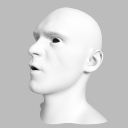
\includegraphics[width=0.3\textwidth]{head_gray_1}\hfill
    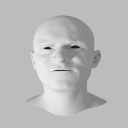
\includegraphics[width=0.3\textwidth]{head_gray_2}\hfill
    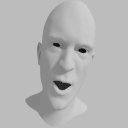
\includegraphics[width=0.3\textwidth]{head_gray_3}
    \caption[Gray head renders]{Head renders with gray background and face textures. A collage of these renders can be seen in figure \ref{fig:head_gray_collage_1}.}
    \label{fig:head_gray_1}
\end{figure}

\begin{figure}[p]
    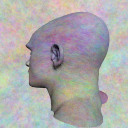
\includegraphics[width=0.3\textwidth]{head_noise_1}\hfill
    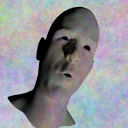
\includegraphics[width=0.3\textwidth]{head_noise_2}\hfill
    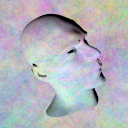
\includegraphics[width=0.3\textwidth]{head_noise_3}
    \caption[Noise head renders]{Head renders with 1/f noise background and face textures. A collage of these renders can be seen in figure \ref{fig:head_noise_collage_1}.}
    \label{fig:head_noise_1}
\end{figure}

\begin{figure}[p]
    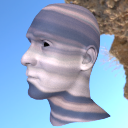
\includegraphics[width=0.3\textwidth]{head_material_texture_1}\hfill
    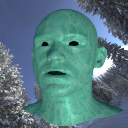
\includegraphics[width=0.3\textwidth]{head_material_texture_2}\hfill
    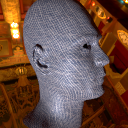
\includegraphics[width=0.3\textwidth]{head_material_texture_3}
    \caption[Non-realistic head renders]{Head renders with realistic background textures and non-realistic face textures. A collage of these renders can be seen in figure \ref{fig:head_material_texture_collage_1}.}
    \label{fig:head_material_texture_1}
\end{figure}

\begin{figure}[p]
    
\includegraphics[width=0.3\textwidth]{dummy1}\hfill
    
\includegraphics[width=0.3\textwidth]{dummy1}\hfill
    
\includegraphics[width=0.3\textwidth]{dummy1}
    \caption*{}
\end{figure}

\begin{figure}
    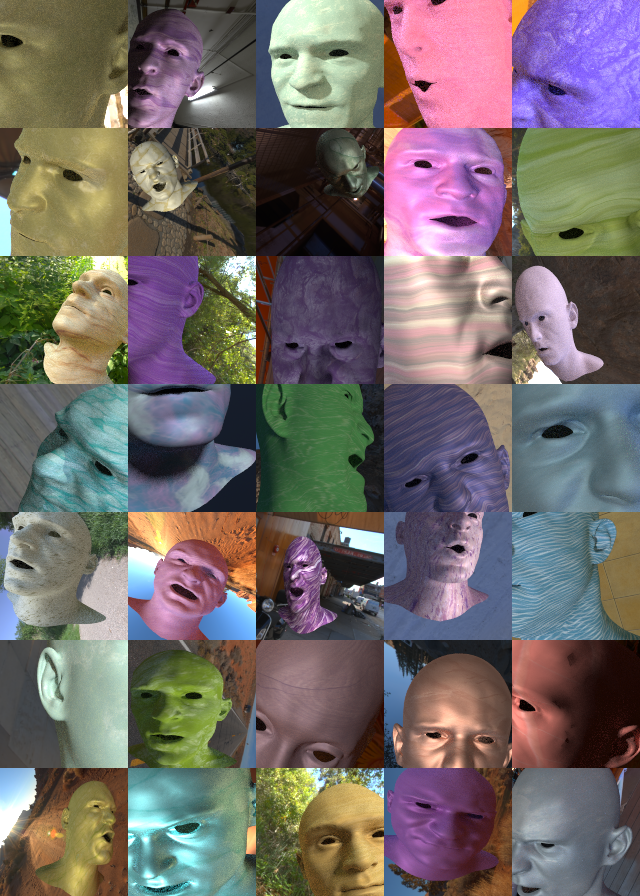
\includegraphics[width=\textwidth]{head_final_texture_collage}
    \caption[Mixed head render collage]{A collage of head renders with realistic background textures and mixed material/realistic face textures. These have the final amount variation between all the randomized rendering parameters.}
    \label{fig:head_final_texture_collage_1}
\end{figure}

\begin{figure}
    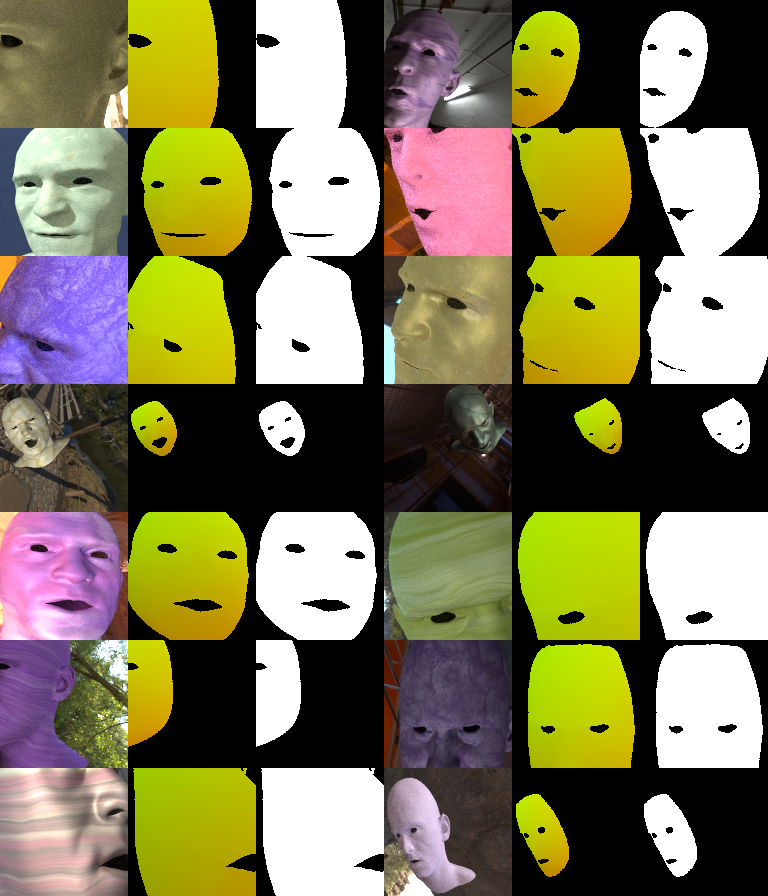
\includegraphics[width=\textwidth]{head_final_triplet_collage}
    \caption[Head triplet render collage]{A collage of head renders with the input, target UV and target mask images. These image triplets formed the training samples.}
    \label{fig:head_final_triplet_collage_1}
\end{figure}

One training sample consisted of three images: the input image, the target UV image, and the target mask image. All the images had a resolution of 128x128 pixels, and they were created from the same randomized rendering parameters. The UV and mask images were rendered with the help of another mask image that segmented out only the frontal face area of the head model. This was done because we were not interested in teaching the network the geometry of the neck or back of the head. Eyes and inside of the mouth with teeth were not included with the original head model, and we did not have assets to model them, so they were left out of the renders. Eyes and inside of the mouth were rendered as black in all three of the training sample images. The resulting image triplets are illustrated in figure \ref{fig:head_final_triplet_collage_1}.

Our rendering loop started by doing all the rendering parameter randomizations. It then rendered the same scene three times, adjusting internal blender settings to generate the different images in the training sample. A random 16 character string was created, and with it, the file names for current rendering sample. Our file naming scheme allowed later the grouping of the rendered files into training samples, whose order could be randomized easily without having to worry about mixing the images.

All the rendering results were stored in floating-point precision. We used the EXR file format with 16-bit floats and ZIP compression. Halving the precision from 32 bits to 16 bits did not affect the results, but reduced the size of the training dataset by a factor of two. The additional built-in ZIP compression reduced file sizes even further, as the UV and mask images were composed of somewhat repeating values. The floating-point precision was essential, especially with the UV images, where the pixel needs to store a real-valued coordinate in the UV space. At first, we used 8-bit precision with the UV images, as is used in the PNG format, and the resulting network did not perform well. In addition, the physically based lighting of the Cycles renderer and \ac{HDR} environment textures generated \ac{HDR} input images. We wanted to save this information so that the data augmentation process would have as much information available as possible.

Antialiasing with 64 samples per pixel was used for input and mask images but disabled for the UV images, where only the center of the pixel was sampled. At the internal facial geometry boundaries, for example between nose tip and upper lip when looked from above, two adjacent pixels could have a considerable distance in the UV space. This is why we reasoned that antialiasing the UV images did not make sense, as it would blur the boundary and generate an invalid UV value. When sampling the pixel centers, it could be possible to find a pixel where the center is inside the model geometry, but part of the pixel is already outside. We did not want to include these pixels in the UV image. We decided to render the mask image with antialiasing which would make these boundary pixels grayscale. These grayscale values could then be thresholded out, and a little bit smaller mask could be created. This mask has pixels that are all 100\% inside the facial geometry and could be used to remove all ambiguous pixels from the UV image.

The rendering speed was about one training sample per second on a modern four-core desktop machine. Most of the time was spent rendering the input image; the UV and mask images were much faster to render in comparison. We kept the sample count per pixel low, at 64, on the input image to keep rendering times in control. Low sample counts caused some noise to be left in the input images, but we reasoned that it does not matter as noise is added anyway in the augmentation process.

Rendering 100 000 training samples would have taken too long on a single machine, so the rendering was offloaded to Aalto Triton and \ac{CSC} Taito computing clusters. The \ac{CPU} utilization of a single Blender rendering process was rather low. It was found out that an optimal combination was to request a job allocation with eight cores and then launch eight separate Blender rendering processes which each was told to use four threads. This way the rendering could reach near 100\% \ac{CPU} utilization, and we witnessed the fastest total rendering times. Each job output the rendered images into the local temporary storage, and after having finished rendering, stored all the images into a tar-archive and sent the file to a shared work directory. After all the jobs had finished, the smaller archives were gathered together and combined into one single large archive. The size of an archive containing 100 000 training samples was around 10 gigabytes.

\section{Neural network design}
\label{sec:net_design}

At the time of starting this project, there were two machine learning Python frameworks that we looked at, \textcite{tensorflow} and \textcite{cntk}. It quickly became clear that the syntax of \ac{CNTK} was simpler, and the examples and tutorials were easier to understand. Back then, Tensorflow did not have an official well-working \ac{GPU} implementation on Windows. In contrast, \ac{CNTK} natively supported \ac{GPU} training without syntax changes on both Windows and Linux. \ac{CNTK} also promised easy-to-use multi-\ac{GPU} training out-of-the-box. The main development of this project was to be done on Windows, and all the training was to be done on Linux servers. So, it was an easy decision to go with the \ac{CNTK} framework.

\begin{figure}
    %\centerline{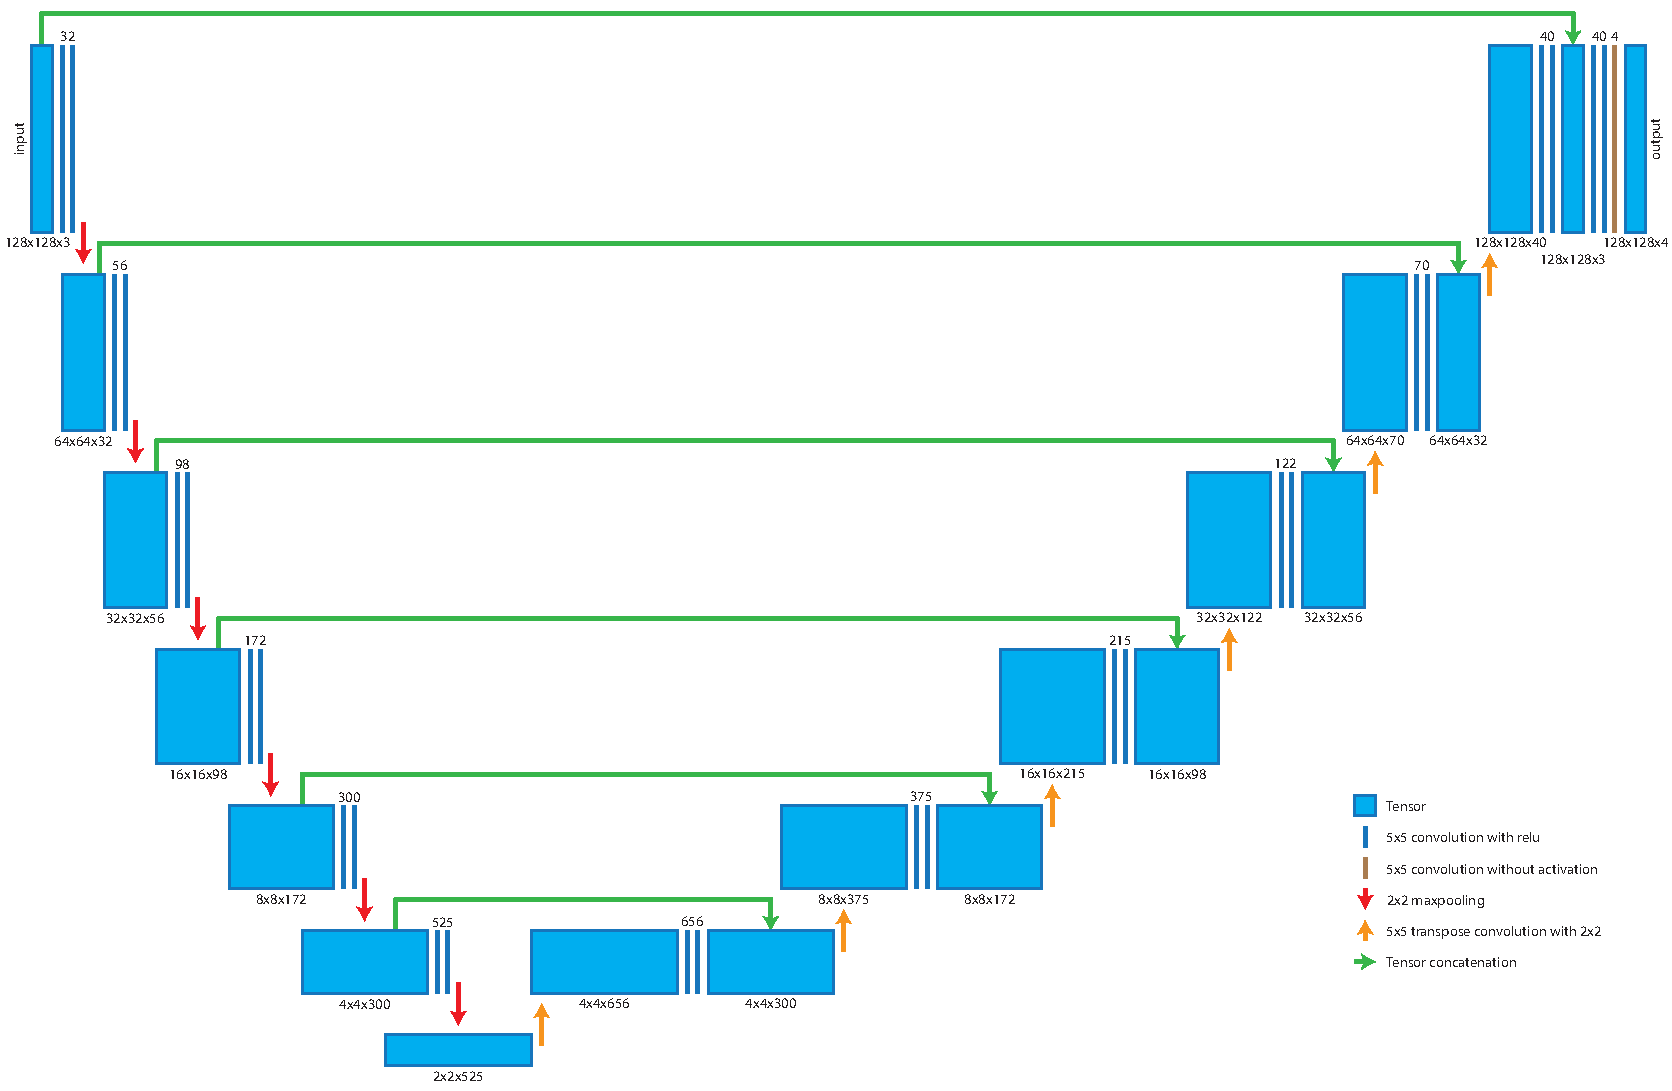
\includegraphics[angle=90,scale=0.85]{uv-net-topology}}
    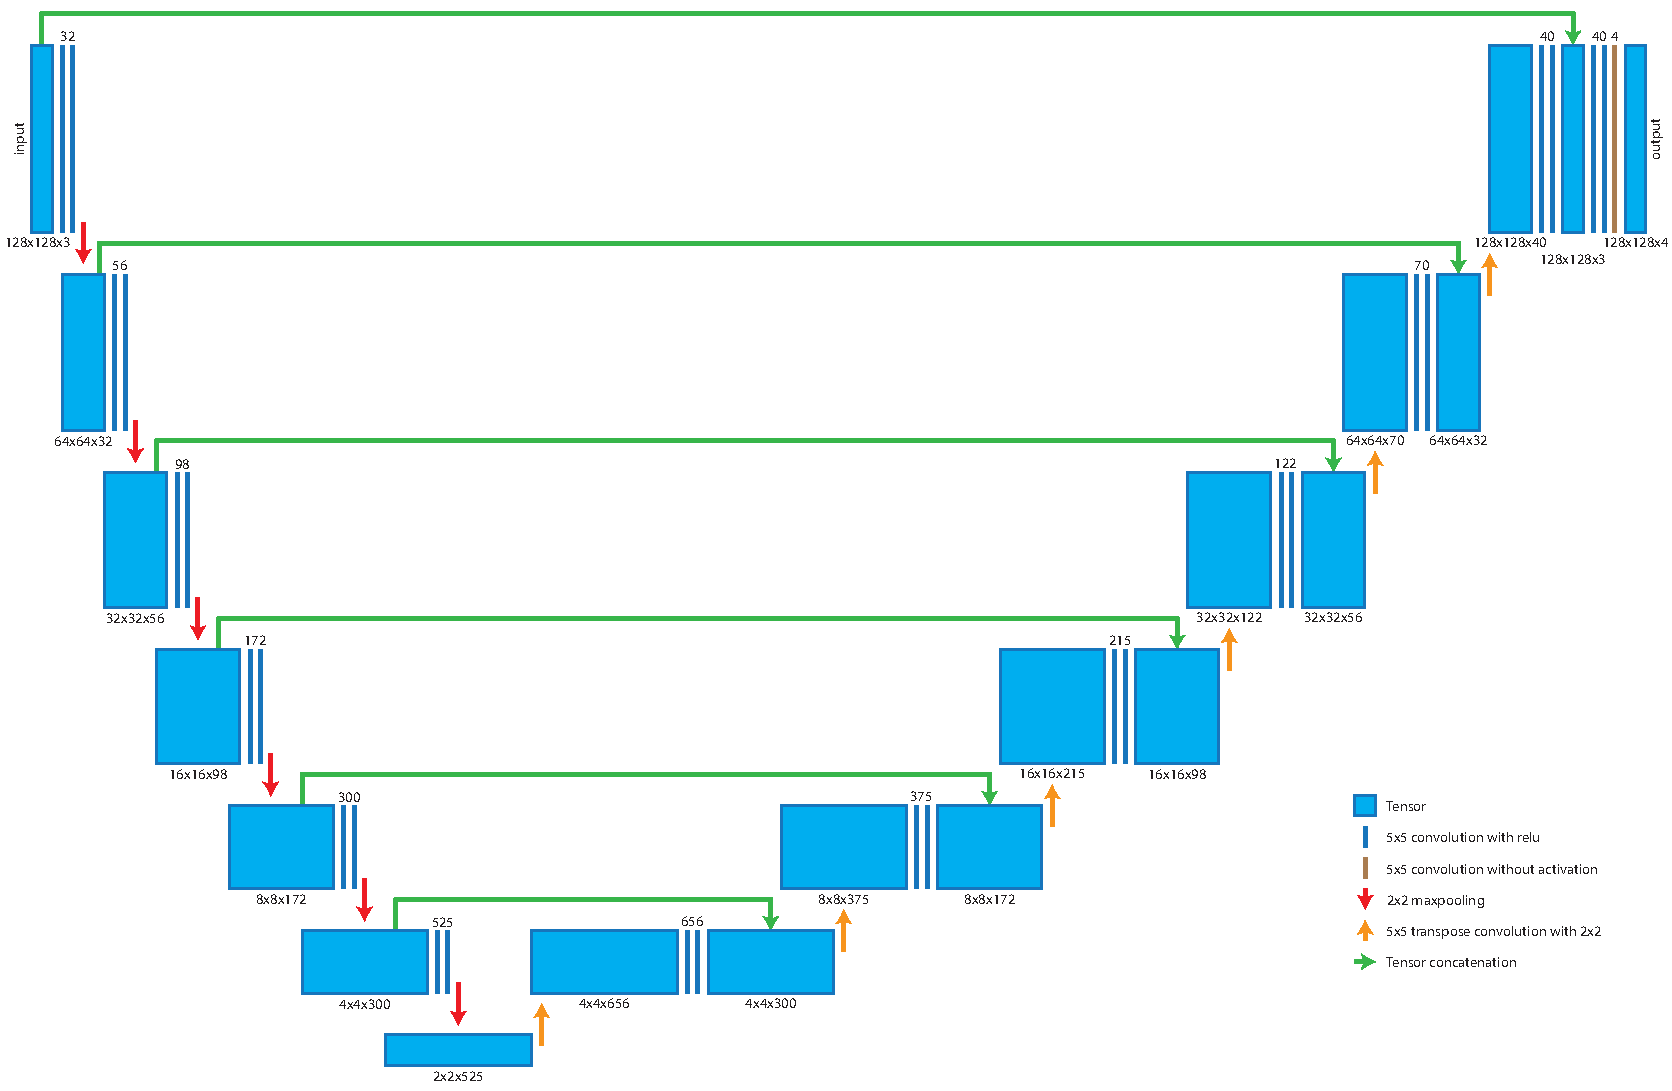
\includegraphics[angle=90,width=\textwidth]{uv-net-topology}
    \caption[Neural network topology]{The final topology of the neural network. It was a fully convolutional network with skip connections between down and upsampling portions. Downsampling was done with max-pooling and upsampling with transpose convolutions. Numbers above the convolution layers convey their feature map sizes.}
    \label{fig:net_top_1}
\end{figure}

Our final network topology is illustrated in figure \ref{fig:net_top_1}. The design relied heavily on the U-net design proposed by \textcite{Ronneberger2015}. The decision to go with the U-net design was influenced by our prior good experiences with it. We decided to call our network UV-net as an homage to its inspirator and because the network did UV mapping. The network was an \ac{FCNN} with skip connections. The input was one image, and the output was three different images of the same size. The skip connections were a vital part of the network, as they were able to preserve the high frequency detail of the input image. Without the skip connections the training process was not able to converge to any satisfactory result.

In figure \ref{fig:net_top_1} the cyan boxes represent the data flowing through the network, the tensors. Tensors are multidimensional arrays of numerical values. In our case, the first tensor was a 128x128x3 floating-point array representing an RGB color image with a resolution of 128x128. The tensor then got processed through the seven levels of the network. At the contracting side of the network, the spatial size of the tensor got reduced but, feature map size increased. In the middle, the tensor size was 2x2x525. At the expanding side, the spatial size was gradually increased, and feature map size decreased. At the end, the network output a tensor with a size of 128x128x4. This included two channels for the UV image and two channels for the two different mask images: normal mask and occluded mask. The skip connections were implemented by first making sure that the spatial dimensions of all tensors on the same level were identical and then just concatenating the tensors together along the feature map axis.

Figure \ref{fig:network_layers_1} illustrates the different layers we used to operate on the tensors. Convolution layers with a filter size of 5x5 were used to extract features from the tensors. For example, the first tensor with three feature maps was convolved with 32 different convolution filters to generate a new tensor with 32 different feature maps. Convolutions used a stride of 1x1, and the input was zero padded to prevent the spatial size reduction of the tensors. The actual downscaling of the tensors was done with 2x2 max-pooling layers \cite{Goodfellow2016}. Each feature map was scanned through looking at disjoint 2x2 pixel areas at a time. Whatever pixel had the highest value was selected. This reduced the spatial dimensions of the tensors by a factor of two. Max-pooling layers also introduced some invariance towards the internal shifting of features. Upscaling of the tensors was done with transpose convolution layers with a filter size of 5x5. These effectively did the same as the convolution layers but in reverse. If a stride larger than one was used, 2x2 in our case, the spatial dimensions of the tensors were increased. The output size would not be the same as if scaled up by a factor of two. This was remedied by just cropping the tensors back to the right size.

\begin{figure}
    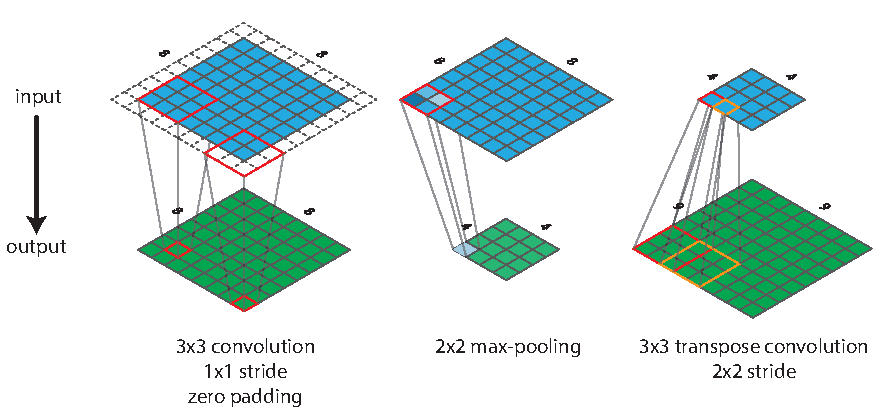
\includegraphics[width=\textwidth]{network-layers}
    \caption[Network layers]{A visualization of the different layers used in the network. Zero padding was used with the normal convolution layers to keep the output same size. Max-pooling layers selected the maximum value inside a 2x2 area, effectively reducing the size by a factor of two. Transpose convolutions with a stride of two were used to upscale. 3x3 convolution filter size is used here for illustration purposes; the final filter size was 5x5.}
    \label{fig:network_layers_1}
\end{figure}

We used exponentially growing feature map sizes as fully convolutional neural networks like ours need large feature map sizes to work well \cite{Ronneberger2015}. We started with 32 initial feature map size and increased that by a factor of 1.75 for every level. On the upscaling side of the network, the feature map sizes were derived from those on the downscaling side by multiplying by 1.25. This was because the network needed more expressivity on the upscaling part for generating dense pixel mappings.

We preferred using two convolution layers in succession with smaller filter sizes to using one convolution layer with a larger filter size. This increased the effective receptive field size of the convolutions while not increasing needed parameter count as much. For example, with two 5x5 filters, the effective receptive field size was 9x9. Two 5x5 filters needed 50 trainable parameters, and one 9x9 filter would have needed 81 trainable parameters.

The convolution layer filter values were prepared using uniform Glorot initialization, described by \textcite{Glorot2010}. All the layers had the bias term enabled. After testing all the available activation functions, we decided to use the \ac{RELU} \cite{Goodfellow2016}. It was fastest to train and gave as good results as the more recent ones, like the \ac{ELU} \cite{Clevert2015}. The last convolutional layer did not have any activation function.

Every part of the network model creation was parameterized. The full network creation code can be seen in listing \ref{appendix:network_code}. This parametrization allowed easy changing of the network topology. Parameters could also be saved to a file and read back later. This made it simple to generate hyperparameter sweep runs on the computing clusters.

\section{Loss function design}
\label{sec:loss_func}

A fully convolutional neural network like ours can be trained in a supervised manner using input/output image pairs. We had hundreds of thousands of these image pairs thanks to the synthetic training data generation process. The network was first given in an input image, and then the generated output images were compared with known ground truth images. The difference between these images could then be used to iteratively update the network parameters to gradually make the output more and more like the ground truth images.

A general overview of the image data flow during processing one training sample and calculating its loss is illustrated in figure \ref{fig:train_sample_1}. The process was started by reading in the current training sample which consisted of input, target UV, and target mask images. The target mask image was thresholded so that the grayscale pixels were turned to black. The target UV image was multiplied with this new slightly smaller target mask image. This removed all the ambiguous border pixels from both the target UV and target mask images.

The original input image and the thresholded target UV and target mask images were then input into the data augmentation process. The process output an augmented input, target UV, and target mask images. In addition, it generated two new mask images: an occluded target mask image and an eroded target mask image. The occlusions in the occluded target mask image reflected the colored occlusions generated onto the augmented input image. The eroded target mask image had a morphological erosion image processing operation applied which increases the size of the black areas and decreases the size of the white areas.

The augmented input image was given to the neural network which generated three output images: result UV, result mask, and occluded result mask. The UV image generated was not masked straight out of the network, so it was multiplied by the augmented target mask to create the final masked result UV image. Result mask and occluded result mask images were left as is.

\begin{figure}
    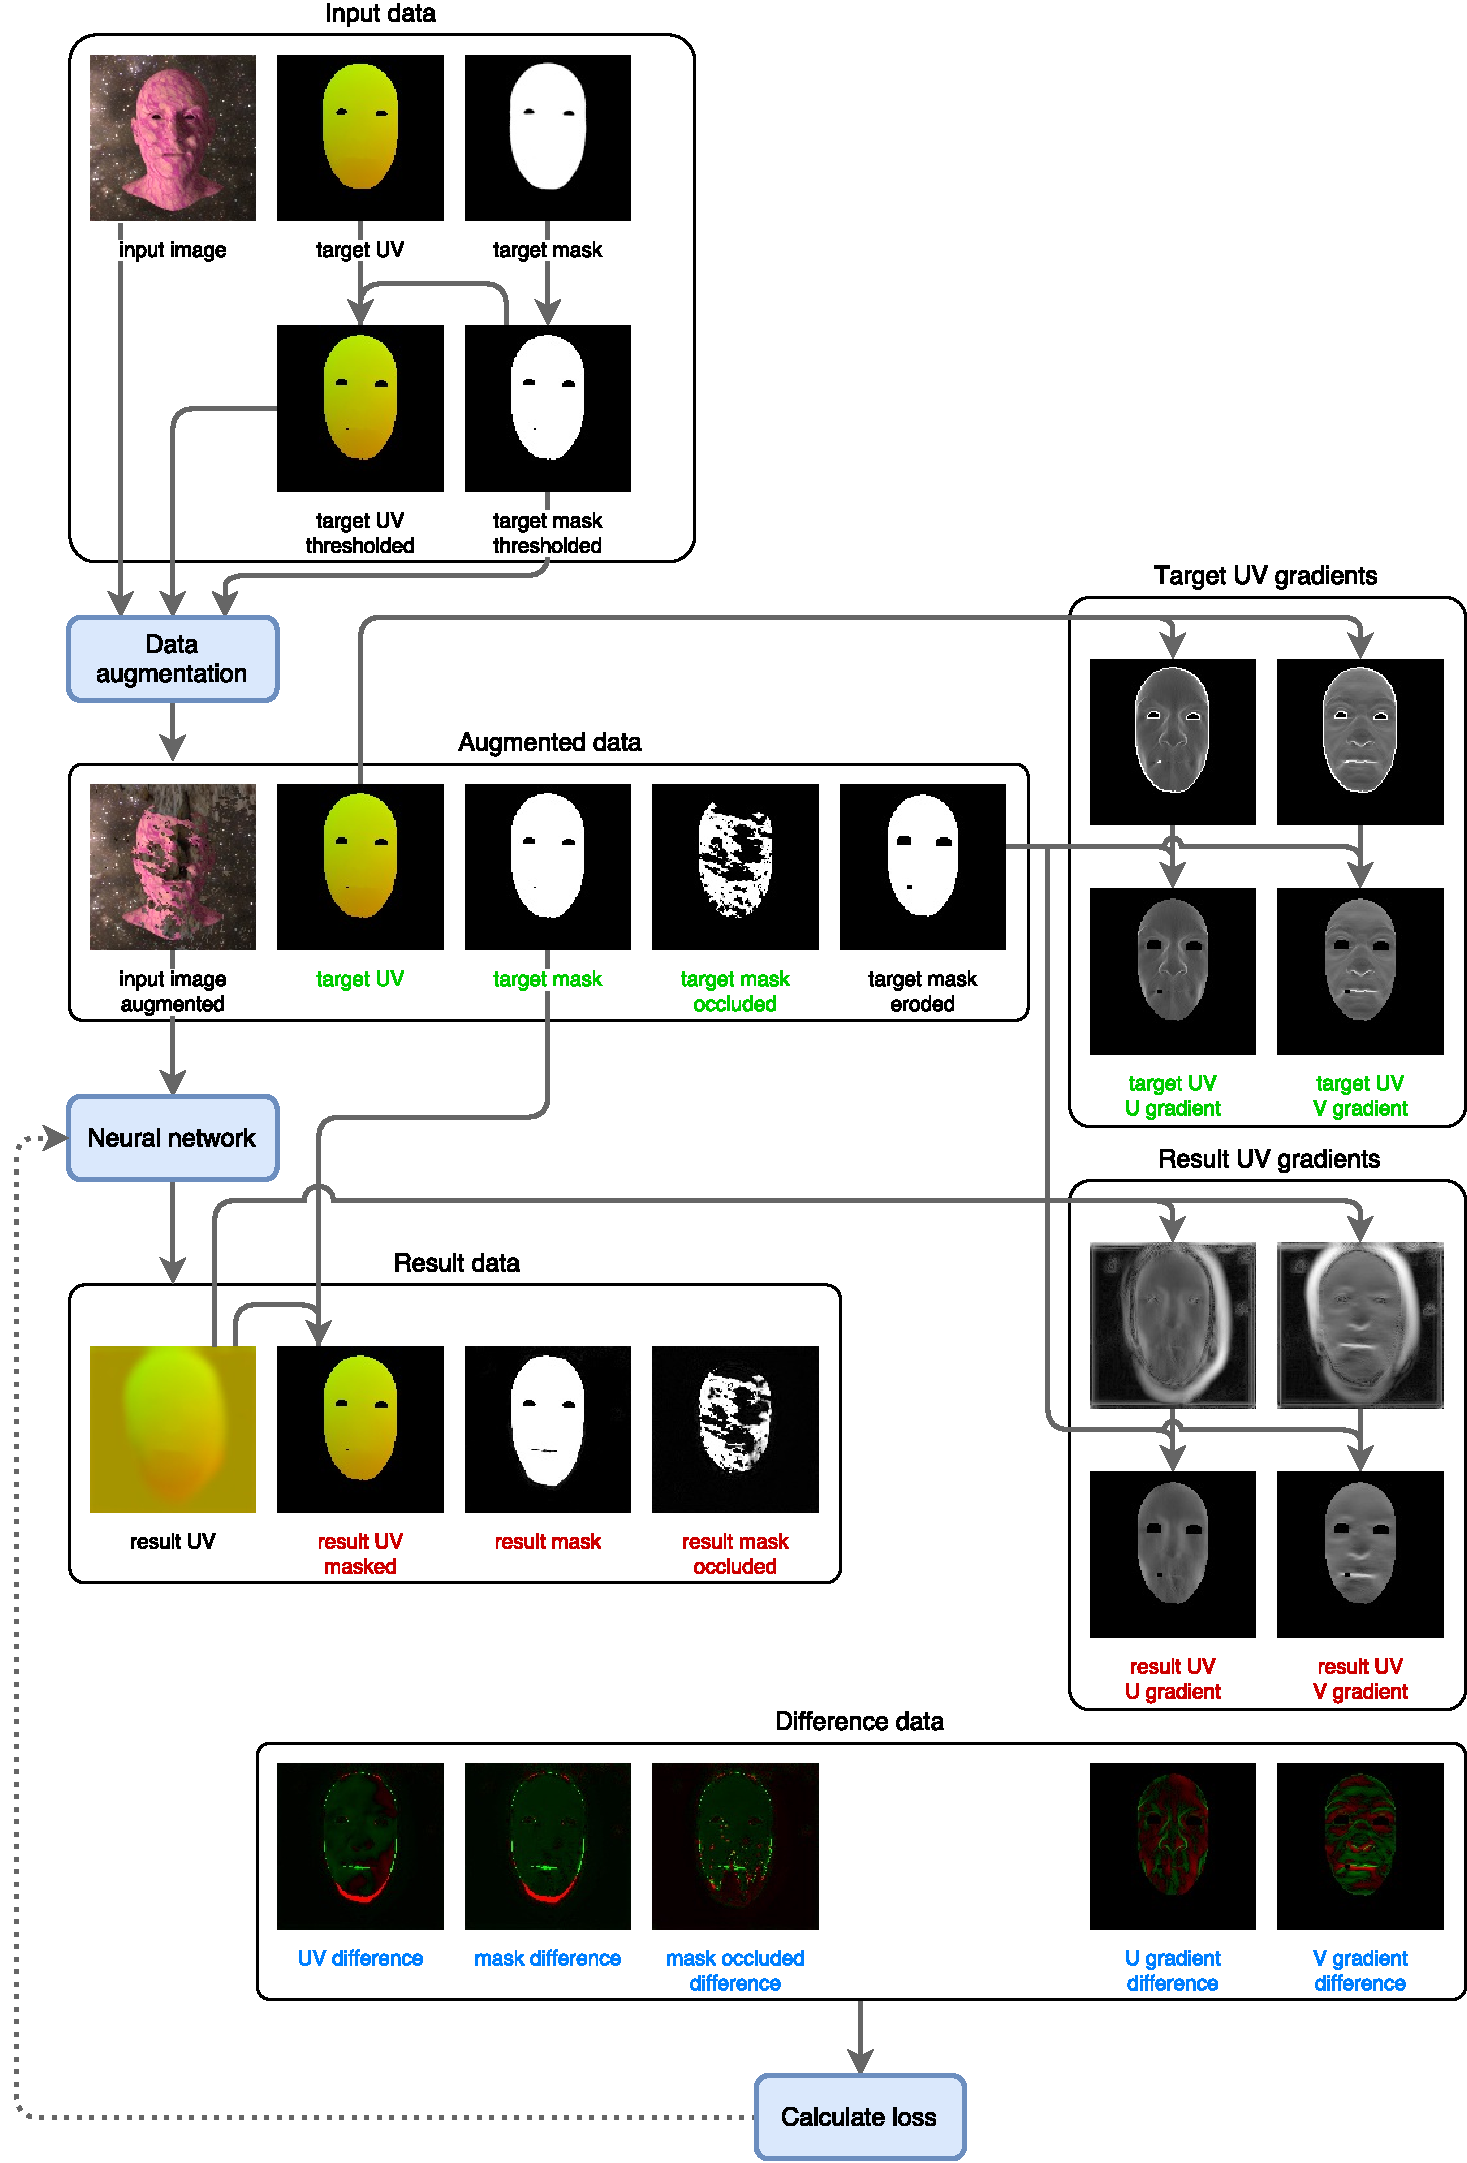
\includegraphics[width=\textwidth]{train-sample}
    \caption[Training sample]{An overview of the data flow when evaluating one training sample. The input data is first preprocessed and then fed to the data augmentation process. From the augmented data, the augmented input image is given to the neural network. The network will output result data which is slightly post-processed. The difference data calculation has not been visualized using arrows but with colors. The result images with red labels are subtracted from the target images with green labels to produce the difference images with blue labels. The actual final loss value is calculated from the difference images with the method illustrated in figure \ref{fig:loss_function_1}. The images on the right side of the figure on this page are the UV gradient images. Gradient images tell how much pixel values change when moving from one pixel to the next. The eroded target mask is used to eliminate large gradient values that exist on, for example, the outer edges of the face.}
    \label{fig:train_sample_1}
\end{figure}

\begin{figure}
    \centerline{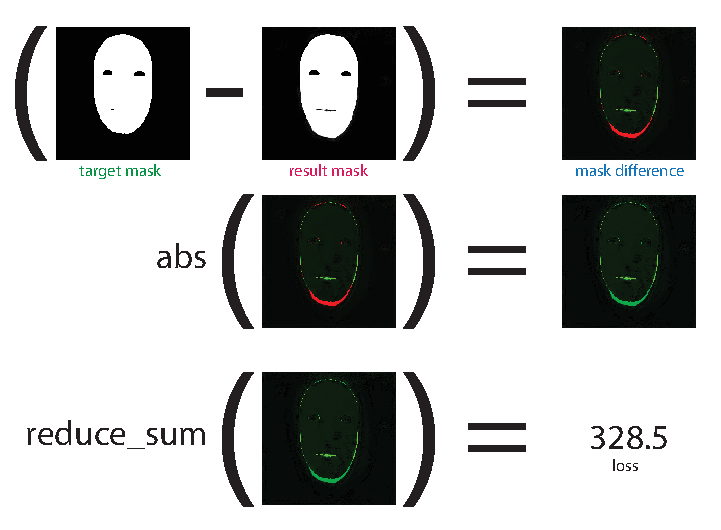
\includegraphics[width=0.75\textwidth]{loss-function}}
    \caption[Loss function]{A visualization of the L1 loss function evaluation for the images. The difference between the images was calculated by a pixel-wise subtraction. Positive values are depicted in green color and negative in red color. The absolute operator turned all pixel values to positive, and the reduce-sum operator summed up all the pixels together to one scalar value.}
    \label{fig:loss_function_1}
\end{figure}

A gradient image describes how much pixel values change between adjacent pixels. We knew that the UV image should mostly have very smooth changes within itself, i.e., no bumpiness or splotchiness in the gradient images. This is because the UV color mapping process inherently generates smoothly varying colors from the smooth UV space. Occasional sharp jumps might be generated by, for example, the nose geometry. Because the UV image should be smooth, its gradient image should, therefore, contain only small gradient values and the sum of the pixels in the gradient image should be low. Thus, low gradient image pixel sum could be used as an additional loss term to help steer the training process towards smoother result UV images.

Gradient images were calculated from both the augmented target UV image and the non-masked result UV image. Gradients were calculated in both X and Y directions for both of the U and V channels, which generated four new images. Figure \ref{fig:train_sample_1} depicts the gradients as vector magnitudes for U and V channels using only one image per each. A problem with the gradients was large values at the edges of the face, mouth and eyes. We were not interested in these as they did not introduce any new actionable information to the process. We remedied the problem by multiplying the gradient images with the previously generated eroded target mask image. This had the desired effect of removing the large edge gradient values from the gradient images.

Figure \ref{fig:train_sample_1} labels the images, between which the loss was calculated, with green and red. The final loss value calculation method is shown in figure \ref{fig:loss_function_1}. The difference between two images was calculated by doing a pixel-by-pixel subtraction. In the difference image, green values depict positive values and red negative values. The absolute operation was then applied to the image resulting in positive values only. All the pixel values were summed over the image resulting in one scalar value. A total of seven of these scalar values were produced, and they were summed together to form the final loss value. To summarize, our loss function was an L1 loss of the UV, UV gradient, mask, and occluded mask images. We tried different combinations of L1 and L2 losses and, in the end, the L1 loss always outperformed the L2 loss when it came to the sharpness of the resulting images. The L2 loss tended to produce blurred mask edges and blotches inside the UV mapping. Full code implementation of the loss function can be seen in listing \ref{appendix:loss_code}.

To optimize the loss, we used the Adam optimization method \cite{Kingma2015} provided with \ac{CNTK}. We started with a learning rate of 0.0001 and a momentum of 0.9. After the loss improvements had tapered off, the learning rate was reduced to 0.00001 and momentum increased to 0.99. Also, the magnitude of the noise augmentation was gradually decreased down to zero during the training process.

\section{Data augmentation process}
\label{sec:data_aug}

\begin{figure}
    \subfloat[none]{\label{fig:augmentations_1a}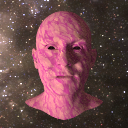
\includegraphics[width=.25\textwidth]{head_augment_none}}\hfill
    \subfloat[rotate]{\label{fig:augmentations_1b}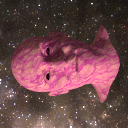
\includegraphics[width=.25\textwidth]{head_augment_rotate}}\hfill
    \subfloat[shuffle]{\label{fig:augmentations_1c}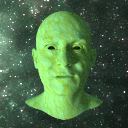
\includegraphics[width=.25\textwidth]{head_augment_shuffle}}\hfill
    
    \subfloat[exposure and \newline gamma]{\label{fig:augmentations_1d}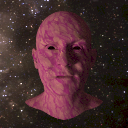
\includegraphics[width=.25\textwidth]{head_augment_expgamma}}\hfill
    \subfloat[noise]{\label{fig:augmentations_1e}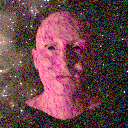
\includegraphics[width=.25\textwidth]{head_augment_noise}}\hfill
    \subfloat[occlusion]{\label{fig:augmentations_1f}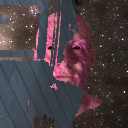
\includegraphics[width=.25\textwidth]{head_augment_occlusion}}\hfill
    
    \centering
    \subfloat[all]{\label{fig:augmentations_1g}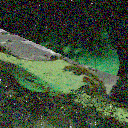
\includegraphics[width=.25\textwidth]{head_augment_all}}
    \caption[Input image augmentations]{Examples of different types of input image augmentations. The final image \protect\subref{fig:augmentations_1g} is the same as \protect\subref{fig:augmentations_1a}, but with all augmentations at their extreme.}
    \label{fig:augmentations_1}
\end{figure}

Without data augmentation, the network did overfit quite quickly. That is, the network learned the training dataset well, but would not generalize to test or real-world images. Data augmentation expanded the existing training dataset many times over. We were able to train a network continuously for ten days without overfitting by combining all our augmentation methods shown in figure \ref{fig:augmentations_1}: rotate, shuffle, exposure, gamma, noise, and occlusions. If the input image in figure \ref{fig:augmentations_1} is compared to the final image with all the augmentations enabled, it is evident that the modifications to the original image could be drastic.

Rotation augmentation (see figure \ref{fig:augmentations_1b}) randomly picked a rotation of 0, 90, 180, or 270 degrees. The input, UV, and mask images were rotated. It should be noted that flip augmentations could not be used in our method, as, for example, flipping along the vertical axis would have made the UV mapping ambiguous. This was not a problem with rotations. The shuffle augmentation (see figures \ref{fig:augmentations_1c} and \ref{fig:head_augment_shuffle_collage_1}) separated the RGB color channels of the input image, shuffled them randomly, and then combined them back into a new image. This effectively increased the training dataset size by a factor of six. The shuffling was done on per color channel, not per pixel. The exposure augmentation multiplied the input image with a random number. The gamma augmentation raised the input image to a random power. These two were used to increase the brightness variation of the input image (see figures \ref{fig:augmentations_1d} and \ref{fig:head_augment_expgamma_collage_1}). The noise augmentation (see figures \ref{fig:augmentations_1e} and \ref{fig:head_augment_noise_collage_1}) added Gaussian noise with random magnitudes to the input image. This was one of the most important augmentations as it made the model much less prone to overfitting. Adding noise made the model generalize better, be less sensitive to small variations in input, and aided the training process to avoid local minima.

\begin{figure}
    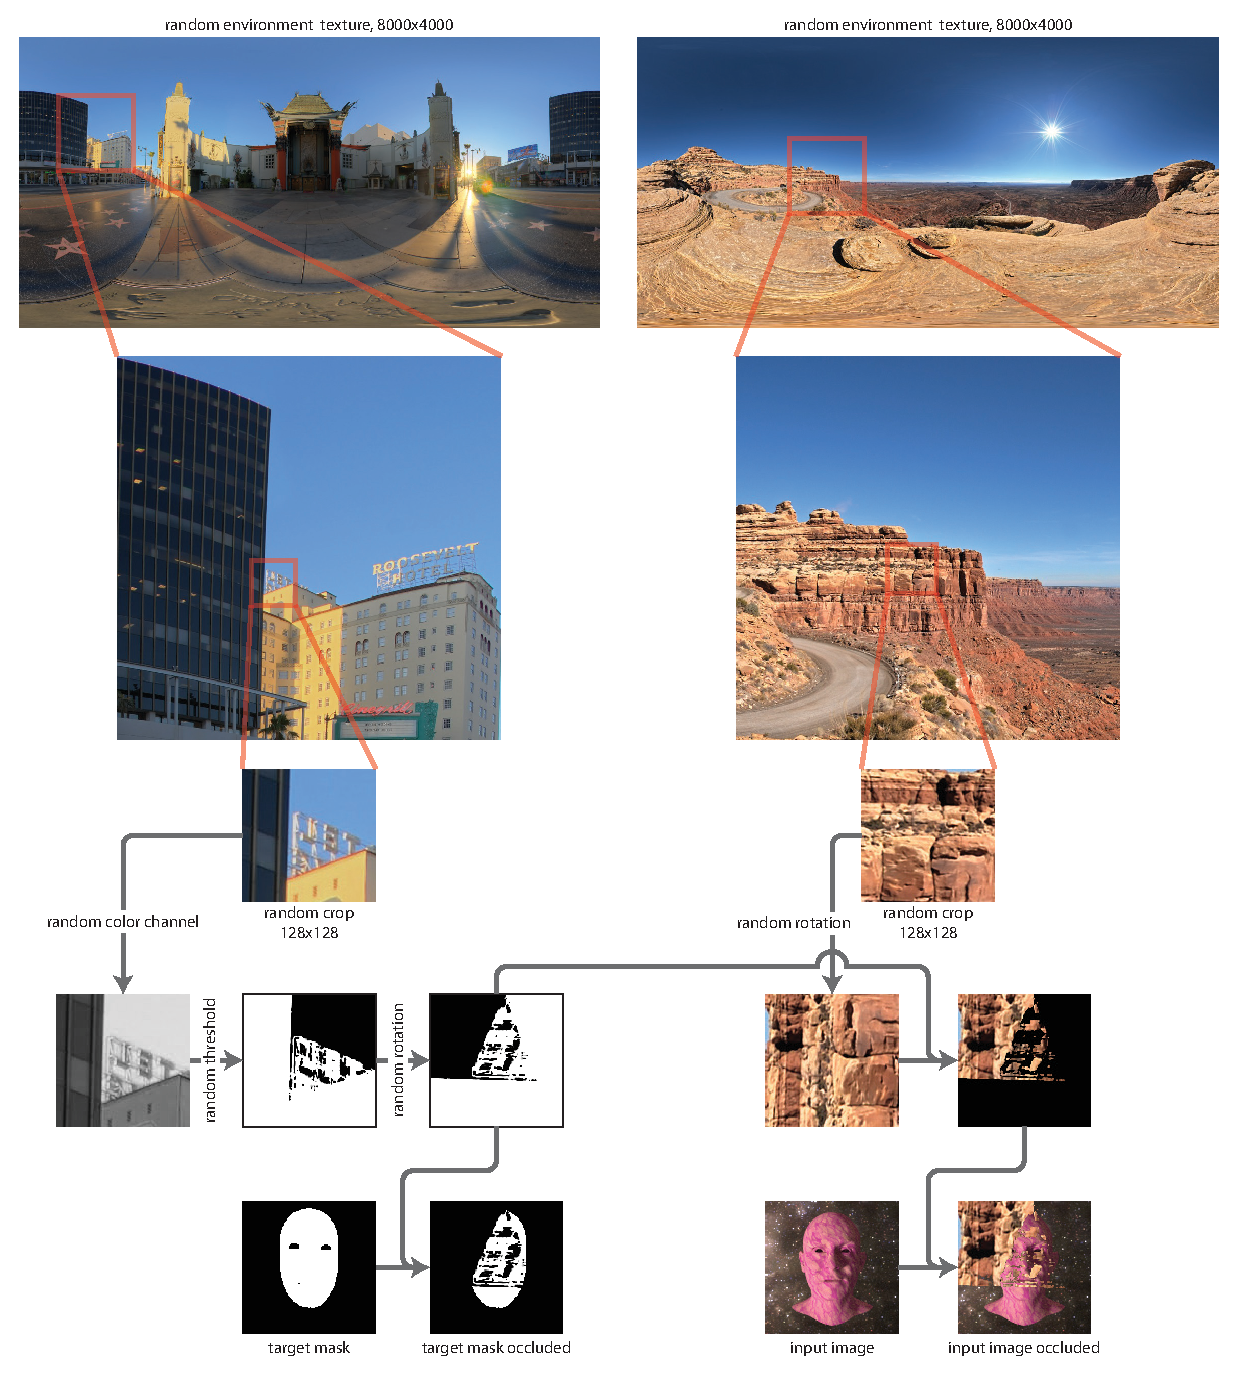
\includegraphics[width=\textwidth]{occlusion-gen}
    \caption[Occlusion generation]{An overview of the occlusion generation process. Two environment textures were selected at random, and a small random area was selected from each of them. These two small images were then used to create the occlusion mask and a color for it.}
    \label{fig:occlusion_gen_1}
\end{figure}

As we evaluated the results, we noticed that any occlusion in front of the face usually degraded the mapping results considerably, usually completely breaking the tracking. Occlusions were, for example, long hair, beards, mustaches, sunglasses, hats and random objects. We did not have assets to add these to the training data, and it would have been infeasible to try to model every kind of possible occlusion. The only way to try to fix this was to add occlusions to the training data, on-the-fly, using augmentation.

Adding rectangular occlusions to the training data, filled with either solid colors or noise, did not improve results. These tended to bias the network to detect every occlusion as a rectangular one. Instead, we decided to use a method that would generate more natural-looking occlusions. The general overview of our method is shown in figure \ref{fig:occlusion_gen_1} and examples of results in \ref{fig:head_augment_occlusion_collage_1}. We obtained 50 \ac{HDR} environment textures from \textcite{sibl}. The textures were of very high resolution, 8000x4000 being the most common one. First, we selected two random pictures from the set. Then, we independently selected a random 128x128 crop from each. The first crop would be used to generate the occlusion mask and the second one would be used to apply color to the mask. This two-step approach was used to increase the randomness of the process, as the mask and its resulting color were not linked together.

\begin{figure}
    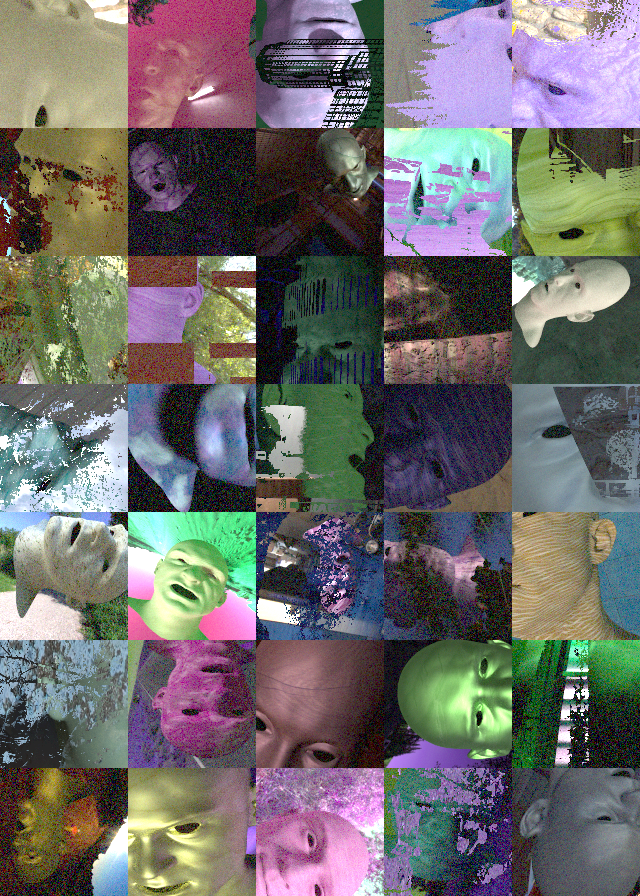
\includegraphics[width=\textwidth]{head_final_texture_augmented_collage}
    \caption[All augmentations collage]{A collage of head renders with all the augmentations applied. Images like these were ultimately fed to the network in the training process. Figure \ref{fig:head_final_texture_collage_1} is the same collage without any augmentations.}
    \label{fig:head_final_texture_augmented_collage_1}
\end{figure}

\begin{figure}
    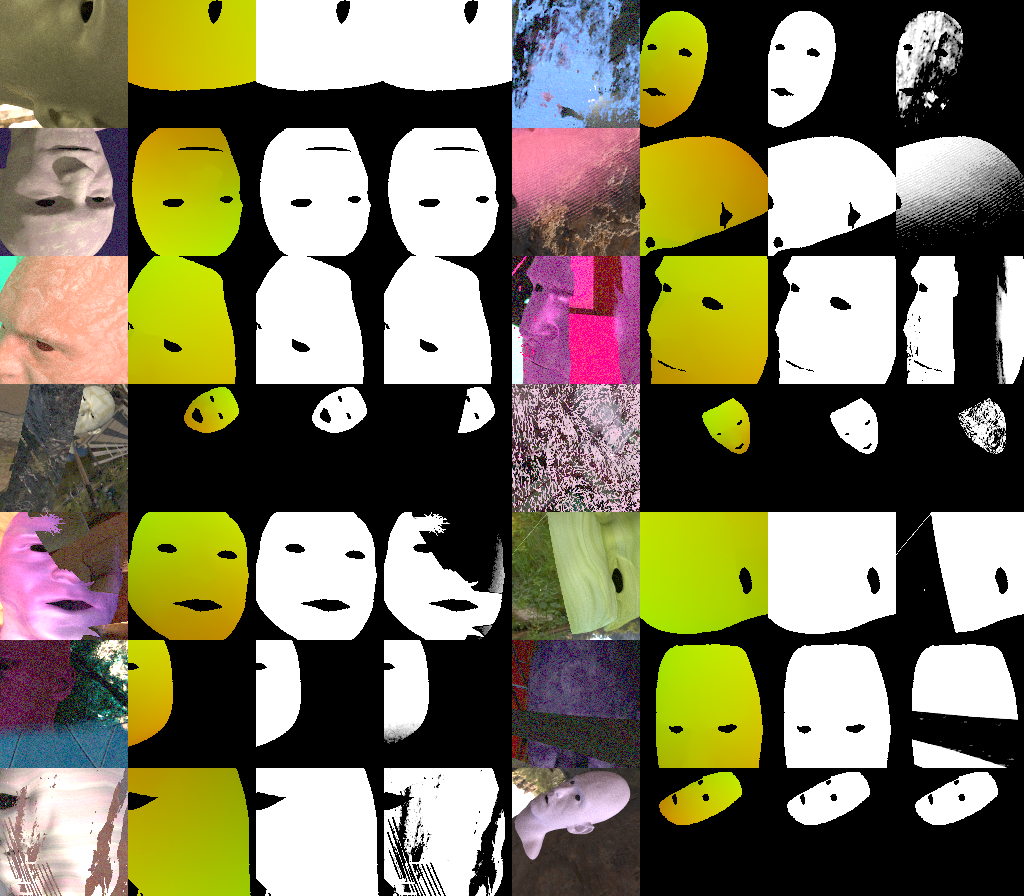
\includegraphics[width=\textwidth]{head_final_triplet_augmented_collage}
    \caption[All augmentations triplet collage]{A collage of augmented head renders with the input, target UV, target mask, and occluded target mask images. The augmentation process mainly touched the input image and generated the occluded target mask. Figure \ref{fig:head_final_triplet_collage_1} is the same collage without any augmentations.}
    \label{fig:head_final_triplet_augmented_collage_1}
\end{figure}

To generate the occlusion mask, a random color channel was selected from the first cropped image and then thresholded. Our thresholding method did not generate binary images, but grayscale images with gradients. This enabled the creation of transparent occlusion masks on top of the input image. The process of creating the threshold image was repeated until the ratio of black to white pixels was within some predetermined range. This range was established by visually inspecting collages of thresholded images and adjusting the target range until there were about equal amounts of black and white. An example of this kind of collage can be seen in figure \ref{fig:occlusion_mask_collage_1}. After successful thresholding, the image was randomly rotated and then multiplied with the target mask to generate the occluded target mask. The random crop from the other texture was also randomly rotated and multiplied with the thresholded image. The resulting color image was then blended over the original input image to create the final occluded input image.

Our rendered data was in floating-point precision, the previously mentioned augmentations were not restricted in range, and our occlusions were based on \ac{HDR} textures. This all meant that our final augmented input image could have values outside the 0.0--1.0 floating-point range. The real-world images that we used for evaluation were in the JPEG or PNG formats. They had 8-bit color channel precision, that is, discrete values between 0 and 255. If a color value like this was converted to floating-point by dividing by 255.0, the result was a value between 0.0 and 1.0 with 255 steps. As a result, for the two final augmentations, we used clipping and quantization. Clipping restricted the color value range between 0.0 and 1.0, and quantization compressed values between this range to 255 distinct values.

A collage of input images with all augmentations applied can be seen in figure \ref{fig:head_final_texture_augmented_collage_1}. Figure \ref{fig:head_final_texture_collage_1} is the same collage without any augmentations. The augmented collage shows that the final training material could be exceedingly non-realistic and hard even for a human to understand. The occlusion method was able to generate a diverse set of colored masks, and sometimes the method even covered the whole face in the image. Figure \ref{fig:head_final_triplet_augmented_collage_1} shows how the whole augmentation process modified the training sample images in general. It can be compared with figure \ref{fig:head_final_triplet_collage_1}. Most of the augmentation methods only touched the input image, the exception being rotation which rotated all images. Occlusion augmentation did not touch the target mask but created a new one, the occluded target mask. This enabled the neural network to detect occlusions while still generating a full, non-occluded, mask image.

\section{Training process}
\label{sec:training_process}

\begin{figure}
    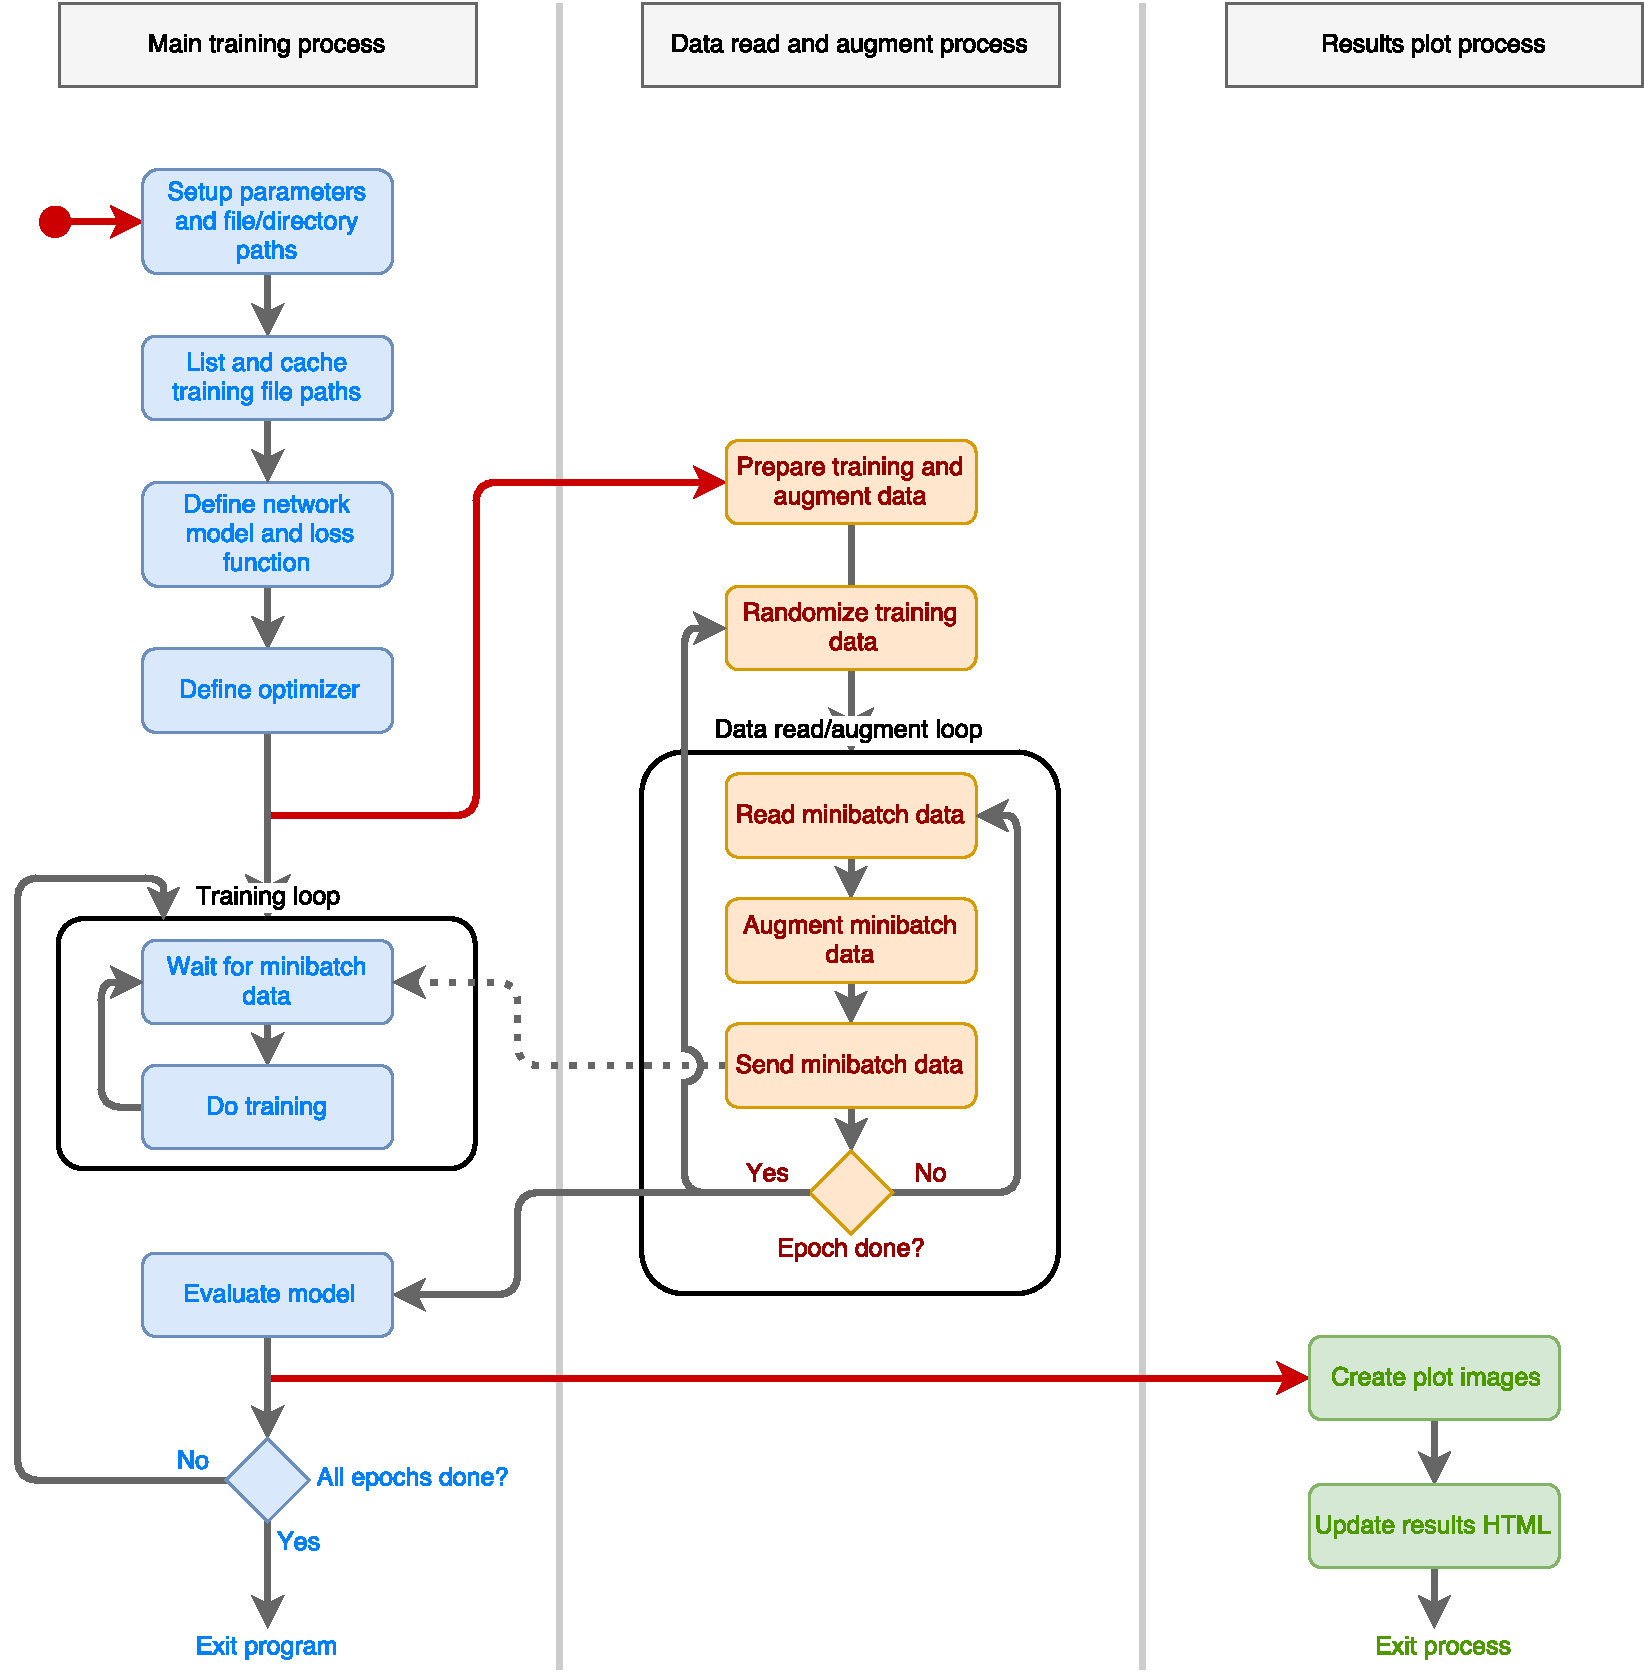
\includegraphics[width=\textwidth]{train-processes}
    \caption[Training software processes]{An illustration of the software processes used during the training and the data flow between them. Red arrows mean starting of a new process.}
    \label{fig:train_processes_1}
\end{figure}

The training process was started by first thinking on a high level what modifications we wanted to do to the network model, loss function, and data augmentation. Because the computing clusters we used had a limit of 20 simultaneous \ac{GPU} jobs, at most 20 different combinations were created. Usually, only a single parameter was changed. Each combination was separately committed to a Git version control repository and tagged with a logical and unique tag name. Then separate jobs, with the tag name as a parameter, were sent to the computing cluster. The first thing the job did was to create a clean working environment and clone the network code from the Git repository with the given tag name. It would also copy and decompress the 100 000 training samples to a local job-specific temporary directory. The job generated a unique run-ID using the tag name and current time. This ID was used to create an output directory to which all the results of the current job would be saved. Doing it this way made it absolutely sure that the network was actually trained with the parameters and training data that it was supposed to. Also, when looking at the results, we could be sure that result files in a specific directory belonged to a specific training run.

After the initial setup was completed, the job launched our Python-based training script. A general overview of the software processes launched at this moment is given in figure \ref{fig:train_processes_1}. The script first listed all files and their paths in the training dataset, grouping them into training sample triplets. \ac{CNTK} was initialized, and it compiled the static graph of the network and readied the target \ac{GPU} for training. The main training loop started to run after that.

All of the data augmentation was implemented in pure Python code, and that proved to be a performance bottleneck. One minibatch contained 40 samples of data and augmenting it took on average the same time as training it. This meant that the \ac{GPU} utilization could only reach 50\% at best. The problem was solved by moving the data augmentation to a separate process using the Python multi-processing module. By doing this, we were able to read and augment the data asynchronously with the training and increase the \ac{GPU} utilization to almost 100\%.

The data reading and augmentation process started by caching the most used files into memory, for example, the environment textures which were used to generate occlusions. The list that contained all the training sample paths was randomized, and the data reading and augmenting loop was entered. The loop started by reading in one minibatch worth of training samples and then augmenting them.  The ready minibatch of data was sent to the main training process by using pipes in the Python multi-processing module. This loop was continued until the end of the training sample path list was reached, or a predetermined number of training samples had been processed. At this point, an epoch was signaled as done. The data reading and augmenting process returned to the sample path list randomization and started the loop again.

Meanwhile, the main training process was reading the minibatches of data from the pipe and sending them to the \ac{GPU} to be processed. This was continued until the epoch done signal was received from the data read and augment process. At this point, the model was evaluated with different evaluation images. The result images were sent to a new plotting process, again, because of Python performance reasons. Plotting all the result images, even after optimizations, took upwards of 30 seconds. The plotting process also updated the result \ac{HTML} file. Next, the main training process returned to the training loop if not enough epochs had been done or the maximum training time limit had not yet been reached. If the limits had been reached, the main process saved the current model parameters to a file and exited.

\section{Visualization methods}
\label{sec:viz_methods}

The generation of the UV mapping allowed us to create various visualizations. They were used to assess the accuracy and stability of the mapping. Accuracy meant how close the generated geometric features matched the actual real geometry and stability how well the features stayed in place while applying the network to video. Any visualization that could be created in the 2D UV space could be easily transferred onto the face. We created four different visualizations: texture projection, inverse texture projection, grid line projection, and grid points projection. Face swapping between two different people and 3D mesh generation should be possible using the mappings, but we did not implement them.

\subsection{Texture projection}

\begin{figure}
    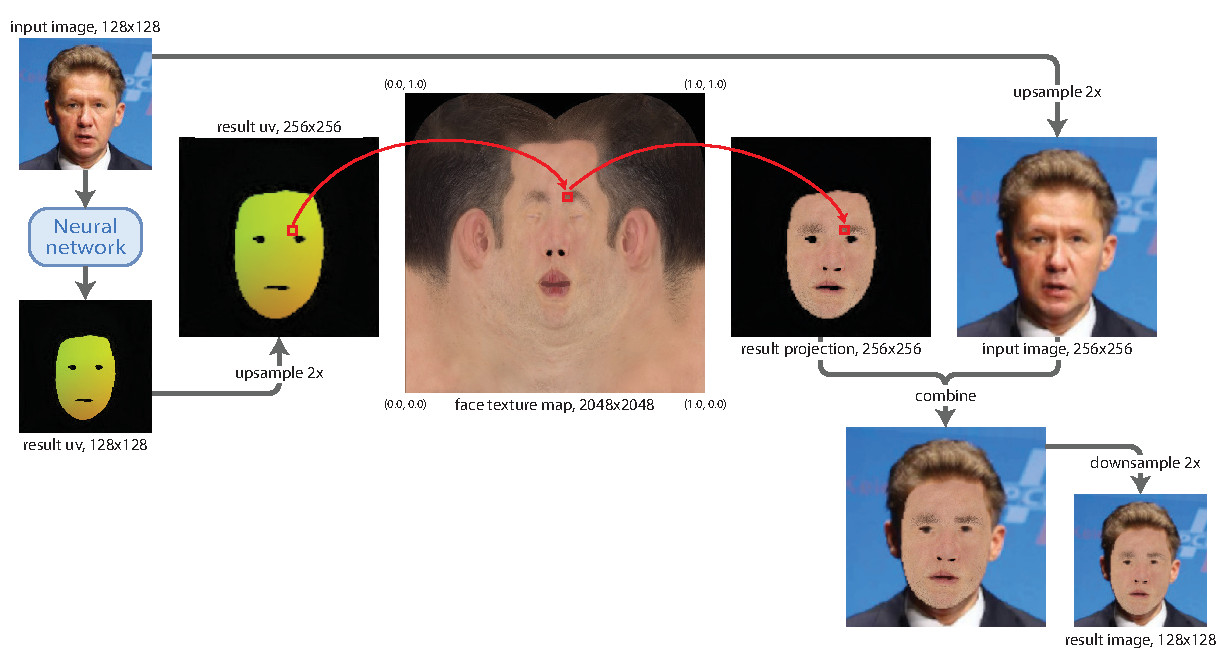
\includegraphics[width=\textwidth]{projection-tex}
    \caption[Texture projection]{Texture projection on the input image. The mapping generated by the network was used to sample a texture, and the result was applied back to the input image.}
    \label{fig:projection_tex_1}
\end{figure}

Texture mapping, using the original texture that came with the model that was used to generate the training data, was an obvious choice for the first visualization. This projection could be used to assess the accuracy of the generated geometry and how similar the looks between the real human and the textured face were. An overview of the texture projection process is given in figure \ref{fig:projection_tex_1}. This method could not take lighting into account, and that is why the textured faces looked flat.

First, a UV map image was created from the input image using the neural network. The UV image was upscaled by a factor of two, and all of its non-black pixels were looped through. Using the UV coordinates encoded to the red and green channels of the pixel, a texture look-up was made. The pixel color value that was read from the texture was written to a new image into the same position as the original pixel in the UV image. The input image was then also upscaled, and the projected image was applied on top of it. Finally, the composite image was downscaled by a factor of two. The images were scaled up and down to introduce a simple antialiasing effect. Without the scaling, the results looked rough and shimmered when applied to a video.

\subsection{Inverse texture projection}

\begin{figure}
    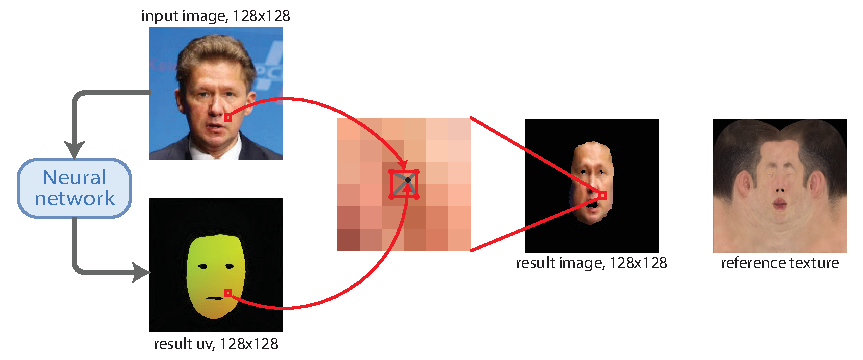
\includegraphics[width=\textwidth]{projection-inv}
    \caption[Inverse texture projection]{Inverse texture projection. The mapping generated by the network was used to transform the input image into the UV domain using bilinear filtering. Result image can be compared to the reference texture.}
    \label{fig:projection_inv_1}
\end{figure}

As the name suggests, the inverse texture projection did the same thing as texture projection, but in reverse. The result was a texture generated using the pixel color values in the input image. The method is illustrated in figure \ref{fig:projection_inv_1}. This visualization could be used to assess how stable the mapping into the UV space was, especially with video input. Even if the subject was making expressions or moving their head around, the facial features mapped into the inverse texture should have always stayed still and not move around.

To begin, the UV mapping was generated from the input image using the neural network. All the non-black pixels in the UV image were looped over. The UV coordinate was read from the pixel and mapped to a location on the result image, basically just by multiplying the UV values, which were between 0.0 and 1.0, by the dimensions of the result image. This resulted in some real-valued coordinates on the result image which did not correspond to exact pixel locations. A color value was read from the input image from the same location as the UV pixel, and this color was applied to the result image pixels using the real-valued coordinate and bilinear filtering. The result image in figure \ref{fig:projection_inv_1} can be compared with the reference texture in the same figure. The reference texture shows how the UV mapping was done with the 3D model we used to generate the training data. The network had learned the UV mapping well if features in the result image were projected to same areas as in the reference texture.

If the subject in the input image was viewed from the side, this visualization should have only projected half of a face. This behavior can be confirmed by looking at row two in figure \ref{fig:results_2}. The inverse texture projection could be developed further to generate a full texture of a human face by analyzing a short video where the head is rotated so that it is visible from all sides at least once. The full texture generation should be possible because no matter which way the face is pictured, a pixel from the same physical point of the face should always map to the same point in the UV space and therefore to the same pixel in the result image. When the head is rotated around, it is seen from all angles, and consequently, the texture generation from a video with some post-processing should be possible.

\subsection{Grid line projection}

\begin{figure}
    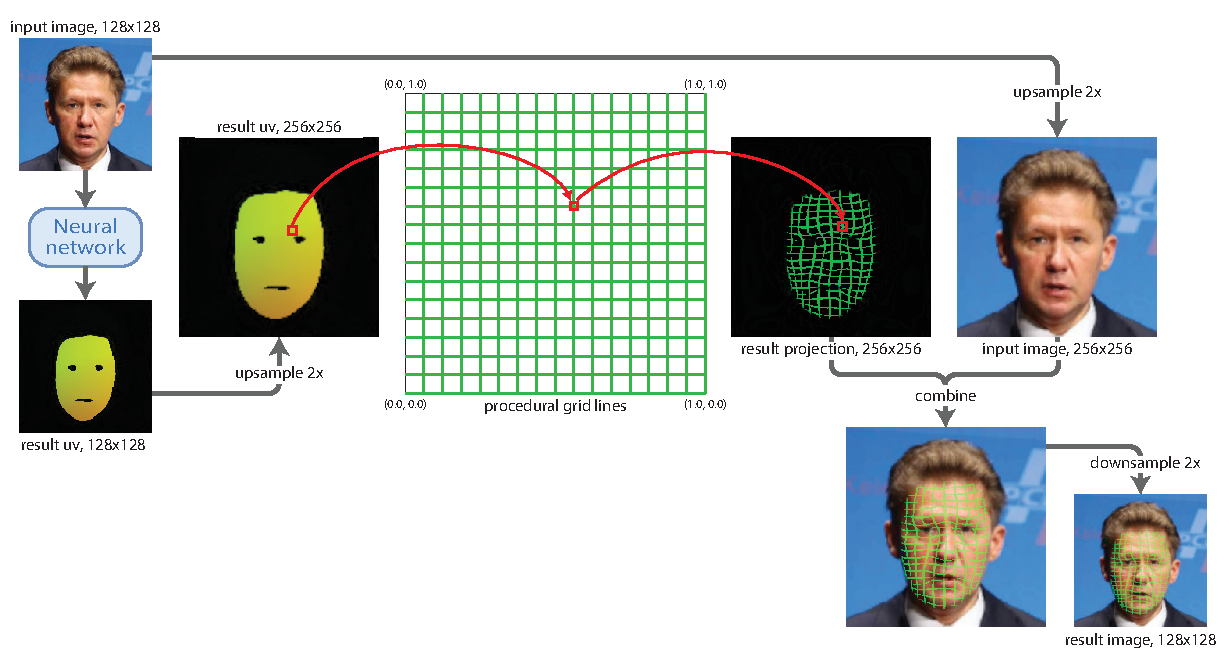
\includegraphics[width=\textwidth]{projection-lines}
    \caption[Grid line projection]{Grid line projection on the input image. The mapping generated by the network was used to sample a procedural line grid, and the result was applied back to the input image.}
    \label{fig:projection_lines_1}
\end{figure}

The grid line projection was similar to the texture projection, with the exception that a grid line texture did not exist but was generated procedurally. This visualization helped to understand the contours of the generated geometry mapping and see how they followed the underlying real geometry. Grid lines were also beneficial when assessing the temporal stability of the mapping when applied to a video.

To create this visualization, a UV mapping was first generated from the input image. The mapping was then scaled up, and the non-black pixels were looped through. The UV values of the pixels were used to sample a procedural grid in the UV space. The grid was created by first multiplying the UV coordinates, which have values between 0.0 and 1.0, by a grid density number larger than 2.0. From the resulting values, the fractional parts were taken. This resulted in values that go again from 0.0 to 1.0 but multiple times in the original range of 0.0 to 1.0. This formed the base of the grid structure. The new repeated UV coordinate could be used to determine if we were near the left or bottom edges of a square, resulting in L-shaped output. When these L-shapes were stacked together horizontally and vertically inside the grid structure, the procedural grid emerged. The density of the grid and the width of the grid lines could be adjusted without any limit. Next, as with texture mapping, the grid lines were sampled to a new image, combined with an upscaled input image, and then scaled down. The up and downscaling was done for simple antialiasing, as the aliasing would have been obvious with the grid line structure.

\subsection{Grid point projection}

\begin{figure}
    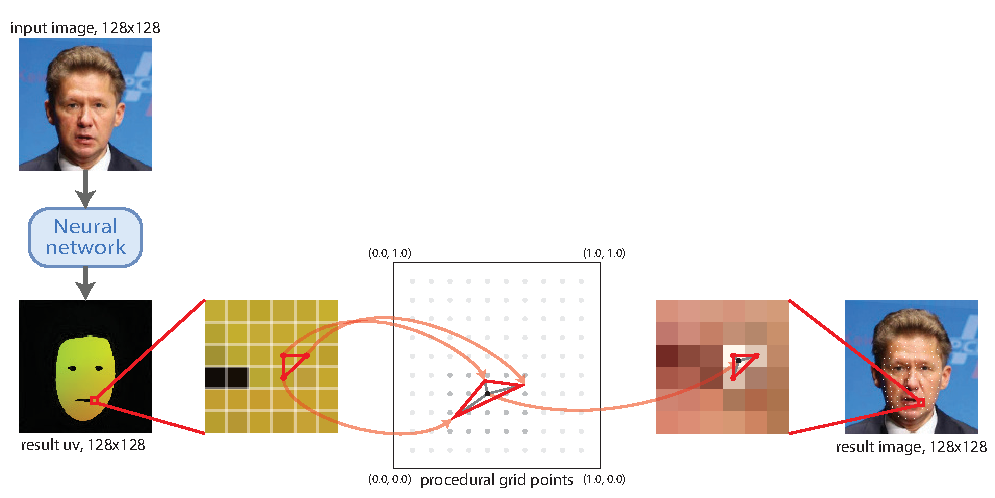
\includegraphics[width=\textwidth]{projection-points}
    \caption[Grid point projection]{Grid point projection on the input image. This could be called the inverse mocap projection. Grid points were procedurally generated and then applied back to the input image using simple filtering.}
    \label{fig:projection_points_1}
\end{figure}

The grid point projection procedurally generated small white dots on top of the input image using the UV mapping. This visualization was created to assess precisely the temporal stability of the results as even little jitter in the dots would have been visible. This projection could also be called the inverse mocap projection because the results resembled faces with the motion capture dots painted on. We implemented the grid point projection somewhat differently compared to the texture or grid lines projections.

The UV mapping was created from the input image using the neural network, but this time the mapping was not upscaled. First, three adjacent UV pixels were selected from the UV image, forming a triangle. The triangle vertices, or pixels, all had 2D UV coordinates. These vertices were projected onto the UV space forming a new, differently shaped, triangle. The UV coordinate values of the vertices, which were between 0.0 and 1.0, were multiplied by a grid density number that was larger than 2.0. Now, it was imagined that the discrete integer coordinates in this scaled space represented the grid points. The size of a subgrid of these integer points, which completely covered the triangle, was then calculated. This subgrid of points was looped through, testing whether any of the points were inside the triangle using a method that returned barycentric coordinates for the point. If a point was found, the color was added to the input image pixels at the same pixel locations where the original UV triangle was formed. The barycentric coordinates for the point were used to determine the amount of color to be added to each of the input image pixels, giving a simple filtering effect. The UV triangles were generated so that the whole area of the UV image was covered.

\section{Results evaluation}
\label{sec:results_eval}

As we iterated over numerous network models, loss functions, and data augmentation methods, we wanted to visually evaluate how the system was performing. We could have used \textcite{tensorboard} to visualize the results and outputs of the training runs, as \ac{CNTK} had built-in support for it. At the time though, Tensorboard did not have all the features needed to visualize the results the way we wanted. We decided to create our own simple \ac{HTML} page that summarized the most important information about the runs and also allowed easy viewing of large amounts of evaluation images. An example of a result web page is shown in figure \ref{fig:browser_results_view_1}.

\begin{figure}
    \centering
    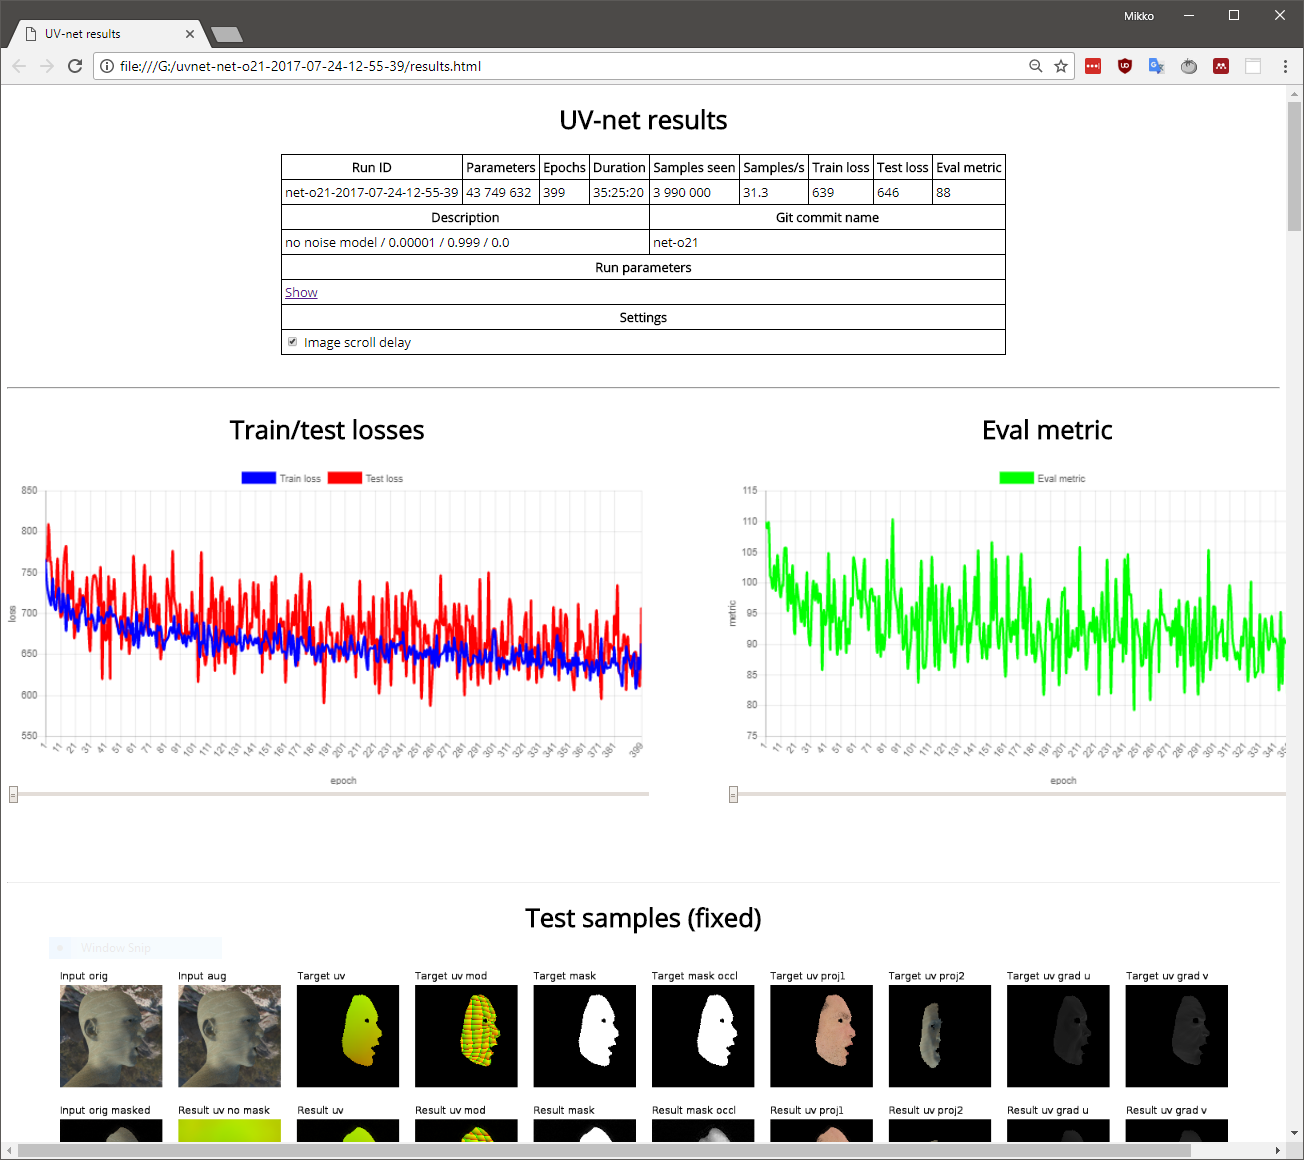
\includegraphics[width=0.95\textwidth]{browser_results_view}
    \caption[Browser-based results viewer]{The browser-based result viewer. The run-specific parameters and values are on the top. The train loss, test loss, and evaluation metric visualizations are in the middle. The epoch specific evaluation images are after that, see figure \ref{fig:eval_image_test_1} for a full example.}
    \label{fig:browser_results_view_1}
\end{figure}

The result page listed the basic information about the particular training run: unique run-ID, total model parameter count, total epoch count, total time used, total samples seen, average samples per second training speed, average train and test loss from last ten epochs, average evaluation metric from last ten epochs, textual description of the run, and the unique Git commit tag name or hash associated with this run. Train and test loss history was plotted in the same graph, which helped to recognize overfitting problems. Evaluation metric history was plotted in a separate graph. Evaluation metric was a simpler absolute error between only the target and result UV images. This metric did not change even if loss function was modified. Loss function values could not be compared between runs if the loss function definition changed. In contrast, evaluation metric values could be compared between all the runs, no matter what. The whole parameter structure associated with the run was also printed on the page, but hidden behind a link. This parameter structure contained every variable that was used to construct the network and could thus be used for verification purposes.

The network was usually evaluated every ten minutes or so, and large evaluation image plots were produced. One example of such an image can be seen in figure \ref{fig:eval_image_test_1}. With these images, we could see how the network performance evolved over time and also cancel training runs that were clearly going nowhere. Per each epoch, the network was evaluated with following as input: six specifically designed synthetic images, one random synthetic image from the current test set, eight specifically selected real-world images, and two randomly selected real-world images. In total, 17 different evaluation plot images were created per epoch. A training run of 72 hours would have around 800 epochs, so in total over 13 000 images could be created.

\begin{figure}
    \centering
    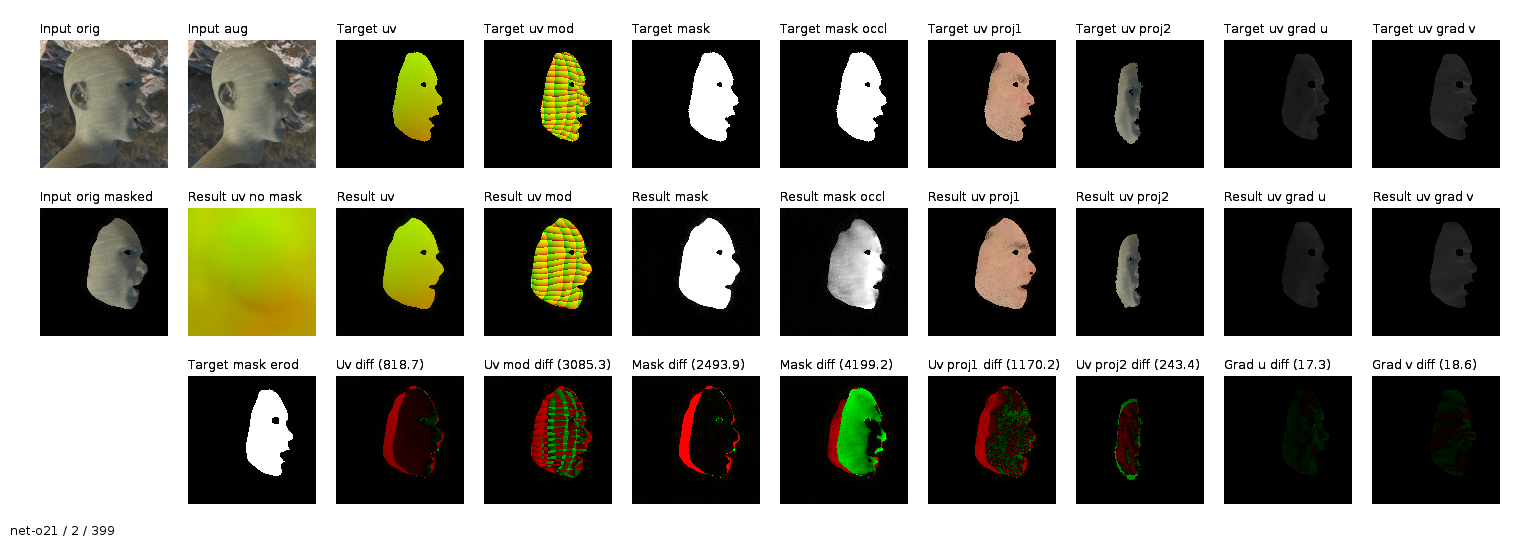
\includegraphics[width=0.95\textwidth]{eval_image_test}
    \caption[Test sample evaluation image]{An evaluation image that was generated using an image from the test set. These were generated for every epoch and could be used to visually track the performance evolution of the network.}
    \label{fig:eval_image_test_1}
\end{figure}

To help to view this large number of images, two things were done. First, the images were saved with a predictable file name pattern of \textit{\{epoch number\}-\{image number\}}. Second, JavaScript, HTML5 canvases, and sliders were used to select and render all these images on a single \ac{HTML} page. Using the sliders, it was easy to go back in time and see how the network performance evolved over time with each of the different evaluation samples. The \ac{HTML} page and all the result images resided on the computing cluster work directory, and it was easy to mount that directory to a local computer using \ac{SSHFS}. This way the downloading of all the evaluation images was prevented and results could be viewed quickly even over a slow connection.

If one moved the slider to see evaluation images of earlier epochs, every epoch image in between would be loaded. This was slow even on computers where the evaluation images were saved locally, not to mention loading them over slow networks. To alleviate this problem, a time delay option was added to the sliders. If one scrolled back in time, the evaluation images would only be loaded after the slider had been stopped for a brief moment. This allowed fast scrolling of evaluation images back in time even over very slow internet connections.
